% =====================================================================
% The Macro Transcension Hypothesis
% Tim Swanson — The Omega Centauri Society / Post Oak Labs
% Target: omegacentauri.me -> arXiv
% Build: pdflatex mth-paper && bibtex mth-paper && pdflatex x2
% =====================================================================
\documentclass[11pt]{article}

\usepackage[margin=1.1in]{geometry}
\usepackage{newtxtext,newtxmath}
\usepackage[round,authoryear]{natbib}
\usepackage{graphicx}
\usepackage{booktabs}
\usepackage{amsmath} % amssymb omitted: newtxmath already provides AMS symbols
\usepackage{tikz}
\usepackage{pgfplots}
\pgfplotsset{compat=1.17}
\usetikzlibrary{arrows.meta,positioning,shapes.geometric}
\usepackage[font=small,labelfont=bf]{caption}
\usepackage{microtype}
\usepackage[colorlinks=true,linkcolor=blue!50!black,citecolor=blue!50!black,urlcolor=blue!50!black]{hyperref}
\usepackage{xcolor}

\newcommand{\msun}{\ensuremath{M_\odot}}
\newcommand{\astar}{\ensuremath{a_\star}}
\newcommand{\kb}{\ensuremath{k_{\mathrm{B}}}}
\newcommand{\specbox}[1]{\par\smallskip\noindent\fbox{\parbox{0.97\linewidth}{\small\textbf{Epistemic status:} #1}}\smallskip\par}

\title{\textbf{The Macro Transcension Hypothesis:\\ Spinning Black Holes in Dense Stellar Clusters as Thermodynamic Attractors for Advanced Civilizations, with Omega Centauri as an Observational Test Bed}}
\author{Tim Swanson\\[2pt]
\small The Omega Centauri Society / Post Oak Labs\\
\small \texttt{tim@postoaklabs.com}}
\date{August 2026 \\[4pt] \small Draft v1.7 (last revised 2026-08-06) --- first paper of the set; companion to the inward-migration review (Paper B), the Omega Centauri campaign (Paper C),\\ \small the migration economics (Paper D), and the engineered-IMBH systems paper (Paper E);\\ \small prepared for omegacentauri.me}

\begin{document}
\maketitle

\begin{abstract}
\noindent
Most proposed resolutions of the Fermi paradox assume that long-lived technological civilizations either expand outward, perish, or deliberately hide. We develop a fourth alternative, the \emph{Macro Transcension Hypothesis} (MTH): that civilizations which optimize for long-term computation are driven by thermodynamics, rather than preference, toward a specific class of astrophysical environment, namely rapidly spinning massive black holes embedded in dense, old stellar systems, and that the migration and its endpoint are both electromagnetically quiet. The MTH extends the transcension hypothesis of \citet{Smart2012} from planet-scale ``inner space'' to macroscopic black-hole infrastructure, and differs from the aestivation hypothesis of \citet{Sandberg2016} in requiring no waiting strategy: the relevant free-energy and entropy-disposal advantages are available now. We quantify the case in four steps: (i) thin-disk accretion onto a Kerr black hole releases 5.7--42\,per cent of rest-mass energy \citep{BardeenPressTeukolsky1972,NovikovThorne1973}, versus 0.7\,per cent for hydrogen fusion, while magnetically arrested disks extract additional spin energy at effective efficiencies exceeding 100\,per cent of accreted rest mass \citep{Tchekhovskoy2011}; (ii) by the generalized second law \citep{Bekenstein1974}, an event horizon is a thermodynamically ideal entropy sink, and a worked delivery budget (Section~\ref{sec:landauer}) shows the realized erasure cost lands a factor of $\sim 10^{6}$--$10^{9}$ below the CMB-limited Landauer floor once carrier propagation and delivery overheads are charged, with little radiated waste heat; (iii) the Bekenstein--Hawking entropy of a $\sim 2\times10^{4}\,\msun$ black hole corresponds to $\sim 10^{86}$ bits, exceeding any material archive; and (iv) per unit of harvested mass, this architecture outperforms complete fusion of the same fuel by a factor of $\sim 11$--$85$, outperforms Dyson-type stellar harvesting without star lifting by $\sim 80$--$600$ in lifetime energy yield ($\sim 11$--$85$ against a star-lifting economy), and exceeds a solar Dyson swarm by a factor of $\sim 10^{9}$ ($6.6\times10^{8}$ at $2\times10^{4}\,\msun$) in instantaneous Eddington-limited power.

We then identify Omega Centauri (NGC~5139), a $\sim 4\times10^{6}\,\msun$, $\sim$12-Gyr-old stripped dwarf-galaxy nucleus hosting the nearest strong candidate intermediate-mass black hole \citep{Haberle2024Nature}, as the most observationally accessible system satisfying the MTH selection criteria, and present a falsification framework built on six instrument-matched tests: accretion-luminosity limits (JWST, ATCA), mid-infrared waste-heat limits, LISA mass and spin measurements (contingent on a compact-object inspiral occurring in-band during the mission), millisecond-pulsar timing, stellar proper-motion accelerations, and neutrino burst searches (KM3NeT). Current data, including the unresolved tension between a $\geq 8{,}200\,\msun$ kinematic lower bound \citep{Haberle2024Nature} and a $\lesssim 6{,}000\,\msun$ pulsar-timing upper bound \citep{BanaresHernandez2025} and the complete electromagnetic silence of the central object \citep{Mahida2026,Chen2025JWST}, are consistent with both the MTH and the more parsimonious gas-starvation null hypothesis; we state explicitly which forthcoming observations would discriminate between them, and which would falsify the MTH outright. The hypothesis is offered in the falsificationist tradition of \citet{Sandberg2016} and \citet{Dvali2023}: a speculative but physically grounded working model whose value lies in the concrete observational program it motivates.
\end{abstract}

\bigskip
\noindent\textbf{Keywords:} Fermi paradox; technosignatures; SETI; intermediate-mass black holes; Omega Centauri; NGC 5139; Blandford--Znajek mechanism; Landauer limit; transcension; aestivation

\newpage
\tableofcontents
\newpage

% =====================================================================
\section{Introduction}
\label{sec:intro}

The Fermi paradox, in its modern form \citep{Hart1975,Tipler1980,Webb2015,Cirkovic2018,Forgan2019}, rests on an expansionist premise: that at least some technological civilizations should grow outward across interstellar distances, and that such growth, sustained for even a small fraction of galactic history, would be conspicuous. The premise is quantitatively robust. Self-reproducing probe architectures permit galaxy-scale colonization in $10^{6}$--$10^{8}$ years \citep{Tipler1980,Freitas1982}, intergalactic expansion is energetically cheap for a mature civilization \citep{Armstrong2013}, and surveys for the waste heat of large-scale energy harvesting have returned null results across $\sim 10^{5}$ galaxies \citep{Wright2014,Griffith2015}. The observed silence therefore demands either that technological life is extremely rare, that it reliably destroys itself, or that the expansionist premise is wrong.

A minority tradition in the literature attacks the premise itself. \citet{Smart2012} proposed the \emph{transcension hypothesis}: that the developmental trajectory of intelligence points not outward but inward, toward ever denser, faster, and more efficient configurations of matter and energy (``STEM compression'' of space, time, energy, and matter), terminating, in Smart's telling, at black-hole-scale densities and an effective exit from the observable universe. \citet{Sandberg2016} proposed the \emph{aestivation hypothesis}: that civilizations which value computation should defer it to the far future, when the cosmic microwave background (CMB) has cooled and each erased bit costs less free energy, and should therefore be dormant now. Both proposals share a key insight, that the thermodynamics of computation is the correct lens through which to predict the behaviour of mature intelligence, and both have been criticized on physical grounds. Smart's mechanism for leaving the universe is not specified in testable form, and the aestivation argument was shown by \citet{Bennett2019} to rest on a thermodynamic error: free energy not harvested now is largely lost, not banked, so a computation-maximizing civilization should collect resources now even if it spends them later.

This paper develops a third member of that family, which we call the \emph{Macro Transcension Hypothesis} (MTH). Its core claim is that the inward trajectory identified by Smart has a concrete, macroscopic, observationally accessible destination in ordinary astrophysics: rapidly spinning massive black holes embedded in dense, dynamically old stellar systems. No new physics, no exit from the universe, and no multi-gigayear dormancy are required. The advantages that drive the migration (accretion power at up to $\sim$60 times the mass-energy efficiency of fusion, an event horizon serving as an entropy sink of unlimited capacity, information storage at the Bekenstein--Hawking density, and gravitational time dilation as a controllable computational resource) are all available in the present epoch, and all follow from textbook general relativity and black-hole thermodynamics \citep{MTW1973,BardeenPressTeukolsky1972,Bekenstein1973,Bekenstein1974}. The hypothesis predicts that the most advanced civilizations remain present but electromagnetically invisible, because maximum computational efficiency, viewed from outside, looks like silence.

The MTH would remain idle philosophy if it did not select targets. The selection criteria (a massive black hole of modest depth, intermediate rather than supermassive; a dense retinue of low-mass stars as fuel; dynamical age sufficient for any migrating civilization to have arrived and matured; and a quiescent electromagnetic environment) converge on a short list of Galactic systems, at the top of which sits Omega Centauri ($\omega$~Cen, NGC~5139): the Milky Way's most massive globular cluster, widely interpreted as the stripped nucleus of an accreted dwarf galaxy \citep{HilkerRichtler2000,BekkiTsujimoto2019,Ibata2019}, host to $\sim 10^{7}$ stars of mean age $12.08 \pm 0.01$~Gyr \citep{Clontz2024}, and, since the detection of seven fast-moving stars within its central 3~arcsec, host to the strongest current candidate for an intermediate-mass black hole (IMBH) in the Galaxy \citep{Haberle2024Nature}. That candidate is simultaneously the subject of a sharp observational controversy: combined stellar-kinematic and millisecond-pulsar-timing analysis places a $3\sigma$ upper limit of $\sim$6,000\,\msun{} on any central point mass \citep{BanaresHernandez2025}, formally inconsistent with the kinematic lower bound. And it is electromagnetically dark to remarkable depth: neither $\sim$170 hours of ATCA radio integration \citep{Mahida2026}, nor JWST infrared photometry \citep{Chen2025JWST}, nor a $\sim$290~ks Chandra exposure \citep{Haggard2013} detects any accretion signature. Every element of this situation (a contested central mass, perfect electromagnetic silence, an imminent decisive instrument in LISA) makes $\omega$~Cen a natural laboratory for testing inward-migration hypotheses, entirely independent of whether the MTH is true.

\subsection{Claims and non-claims}
\label{sec:claims}

Because the argument mixes established physics with speculative inference, we state the epistemic register of each claim explicitly. The paper makes three claims of different strength:

\begin{enumerate}
\item \textbf{(Established physics plus a comparative synthesis.)} Spinning black holes in dense old clusters are, by a wide quantitative margin, the most thermodynamically favourable environments in the present-day universe for long-term, large-scale computation. The ingredient results are established physics; the optimality claim is a synthesis over a stated comparison set (fusion, Dyson-type stellar harvesting, and cold-space computing), defended quantitatively in Section~\ref{sec:thermo} using standard results \citep{NovikovThorne1973,BlandfordZnajek1977,Bekenstein1974,Landauer1961,Lloyd2000}, and is independent of any claim about extraterrestrial intelligence. The ranking of cluster IMBHs above supermassive holes rests partly on strategic rather than thermodynamic criteria (hazard exposure, contested resources), which we treat separately in Section~\ref{sec:whynotsgra}.
\item \textbf{(Speculative hypothesis.)} If long-lived technological civilizations exist and even a subset optimizes for computational capacity, the environments of claim 1 act as attractors, and the resulting migration resolves the Fermi paradox without rare-Earth or doomsday assumptions. This is the MTH proper, stated formally in Section~\ref{sec:hypothesis}. We regard it as less parsimonious than the null hypothesis (technological life is rare or absent) and say so.
\item \textbf{(Observational program.)} Whether or not claim 2 is true, it generates instrument-matched, time-bounded, falsifiable predictions at $\omega$~Cen, several of which will be adjudicated by existing or funded instruments within $\sim$15 years. This program is presented in Section~\ref{sec:falsification}.
\end{enumerate}

We do not claim that $\omega$~Cen hosts a civilization; we do not claim the IMBH is confirmed (it is not); and we do not claim the observed electromagnetic silence is evidence for the MTH, since it is equally consistent with the simpler gas-starvation explanation that we adopt as the null hypothesis throughout.

\subsection{Structure of the paper}

Section~\ref{sec:related} situates the MTH in the literature. Section~\ref{sec:hypothesis} states the hypothesis formally as four postulates. Section~\ref{sec:thermo} develops the quantitative thermodynamic and computational case. Section~\ref{sec:omegacen} reviews $\omega$~Cen and its IMBH evidence, including the current mass tension. Section~\ref{sec:architecture} sketches, at the level of explicitly labelled speculation, the staged architecture by which a migrating civilization would exploit such a system. Section~\ref{sec:falsification} presents the falsification framework and observational roadmap. Section~\ref{sec:discussion} addresses objections, and Section~\ref{sec:conclusion} concludes.

% =====================================================================
\section{Relation to prior work}
\label{sec:related}

\subsection{The expansionist mainstream}

The canonical statements of the Fermi paradox \citep{Hart1975,Tipler1980} treat interstellar expansion as the default behaviour of technological life, an assumption sharpened by \citet{Armstrong2013}, who showed that a single mature civilization could seed every galaxy within several billion light-years using a fraction of one star's output. The ``grabby aliens'' model of \citet{Hanson2021} quantifies the selection effect: if loud (expanding) civilizations exist at any appreciable rate, they dominate the future light cone, and our own early arrival is informative about their density. Observational programs built on the expansionist premise (radio and optical SETI, \citealt{Tarter2001}; waste-heat surveys, \citealt{Dyson1960,Wright2014,Griffith2015}; and the broader technosignature framework, \citealt{Wright2022,SocasNavarro2021,Lingam2021}) have produced consistent null results. Within the expansionist frame, these nulls force the unattractive trilemma of rarity, doom, or concealment.

\subsection{The inward-migration family}

The MTH belongs to a smaller family of proposals holding that mature intelligence migrates down thermodynamic gradients rather than out across space.

\textbf{Transcension.} \citet{Smart2012} argued that the developmental history of complexity on Earth exhibits sustained compression in space, time, energy, and matter (``STEM compression''), and extrapolated to a future in which civilizations engineer environments of black-hole density and disappear from the observable universe. The MTH adopts the compression premise but rejects the terminal step: nothing in known physics permits or requires an exit from the universe, and a hypothesis terminating in unobservable territory cannot be tested. The MTH instead halts the inward trajectory at a macroscopic astrophysical object, an existing massive black hole, where every claimed advantage is calculable and several are observable, which is the sense in which the transcension here is macro.

\textbf{Postbiological migration.} The closest precursor to the present proposal is \citet{CirkovicBradbury2006}, who argued that postbiological civilizations should migrate down Galactic thermodynamic gradients toward the cold outer Galaxy, where computation is cheaper, and that SETI's apparent failure reflects a search aimed at the wrong locations. The MTH shares the thermodynamic-migration logic and the diagnosis of SETI's targeting problem, but identifies a different optimum: the relevant gradient, we argue, is set by the conjunction of energy density, entropy-disposal capacity, and storage density rather than by ambient temperature alone, and its maxima are spinning black holes in dense old clusters rather than the Galactic outskirts.

\textbf{Aestivation.} \citet{Sandberg2016} proposed that civilizations defer computation until the CMB cools, gaining a factor of up to $\sim 10^{30}$ in computations per joule, and so should currently be dormant. \citet{Bennett2019} showed the argument neglects the irreversible loss of free-energy resources not collected promptly: stars burn whether or not anyone harvests them, so maximizers should be active now. The MTH avoids this objection by construction: instead of waiting for a colder universe, it imports a colder-than-CMB entropy sink into the present. Waste entropy crossing an event horizon increases horizon area in accordance with the generalized second law \citep{Bekenstein1974}, at an effective marginal temperature far below the CMB's 2.7~K (Section~\ref{sec:landauer}). An MTH civilization harvests aggressively in the present epoch, consistent with the Bennett--Hanson--Riedel optimality argument, while enjoying much of the efficiency gain that motivated aestivation.

\textbf{Black holes as civilization infrastructure.} The conceit is older than SETI's engagement with it. \citet{Penrose1969} introduced rotational-energy extraction with an advanced-civilization framing, and \citet[\S 33.7]{MTW1973} formalized it as the garbage-dump thought experiment: a civilization lowers its waste to just outside the horizon, releases it, and recovers up to 29 per cent of the rest mass as work. \citet{Thorne1994} staged the same power station for a popular audience, and \citet[\S 12]{FrolovNovikov1998} give the textbook treatment of black holes as energy sources for civilizations. The present series is a completion of that thread. Within SETI proper, several authors have treated black holes as energy sources or computational substrates for advanced intelligence: \citet{Inoue2011} proposed Dyson-type collectors around an accreting supermassive black hole; \citet{Hsiao2021} computed the detectability of a ``Dyson sphere around a black hole'' harvesting disk luminosity; \citet{Opatrny2017} analysed the inverted configuration in which a black hole serves as the cold reservoir of a heat engine run against the warmer sky; \citet{Vidal2011,Vidal2014} argued that black-hole-coupled (``stellivore'') systems are the natural attractor for cosmic intelligence; and \citet{Dvali2023} analysed black holes as quantum information processors for extraterrestrial civilizations, predicting characteristic high-energy neutrino emission from artificial micro-black-hole computers. \citet{Lacki2025} survey the corresponding high-energy SETI opportunity, and the Dyson Minds workshop \citep{Curtis2026DysonMinds} has since brought this thread into mainstream observational planning, recommending anomaly-detection searches of archival WISE, JWST, and EHT data for black-hole-hosted intelligence, with a focus on supermassive hosts. The MTH synthesizes this thread and adds the two elements it has lacked: a \emph{selection theory} specifying which black holes are preferred and why (intermediate-mass, high-spin, cluster-embedded; Section~\ref{sec:selection}), and a named, ranked observational target with a costed test program.

\textbf{Kardashev and his inversion.} The Kardashev scale \citep{Kardashev1964} ranks civilizations by total energy throughput, implicitly rewarding outward expansion. \citet{Barrow1998} proposed the complementary inward scale: mastery over ever-smaller scales of structure. The MTH is the astrophysical completion of Barrow's inversion --- the observation that the universe already provides, free of charge, the densest stable structures that inward mastery could aim at, and that the rational endpoint of a Barrow-type trajectory is therefore relocation rather than fabrication. \citet{Bradbury1999} reached a related conclusion from the engineering side: his Matrioshka-brain analysis shows stellar-powered computation is ultimately limited by radiator area and sink temperature, the constraints an event horizon eliminates.

\subsection{What is new here}

To our knowledge this paper is the first to (i) state the inward-migration resolution of the Fermi paradox as a falsifiable selection theory over real astrophysical objects; (ii) integrate the generalized second law, the Landauer bound, Kerr accretion efficiency, Blandford--Znajek extraction, and Bekenstein--Hawking storage into a single quantitative budget for a civilization-scale computer hosted by an existing black hole; and (iii) attach the resulting predictions to a specific system ($\omega$~Cen) with instrument-matched falsification thresholds and timelines. Each ingredient exists in the literature; the synthesis, the selection criteria, and the test program are new.

% =====================================================================
\section{The hypothesis}
\label{sec:hypothesis}

\specbox{Sections \ref{sec:hypothesis}--\ref{sec:thermo} contain, respectively, a speculative hypothesis stated formally, and established physics offered in its support. The physics in Section~\ref{sec:thermo} stands regardless of the hypothesis.}

We state the MTH as four postulates.

\begin{description}
\item[P1 (Optimization pressure).] Among long-lived technological civilizations, a non-empty subset evolves (by competition, self-modification, or design) toward maximizing long-term computational capacity per unit of controlled resource. (Motivation: computation is the universal currency into which information-processing agents can convert essentially any terminal goal. This is the instrumental-convergence thesis \citep{Omohundro2008,Bostrom2012}, given formal treatment by \citet{BensonTilsenSoares2016}, and the same premise adopted by \citealt{Smart2012} and \citealt{Sandberg2016}. What remains open is the step from convergent instrumental goals in a single agent to a population claim over lineages; P1 asserts only a non-empty subset, the weakest form that step permits.)

\item[P2 (Thermodynamic gradient).] For any such maximizer, the present-day universe contains a strict gradient of substrate quality whose global optima are rapidly spinning massive black holes embedded in dense, old, low-luminosity stellar systems. The gradient is set by four independent physical quantities: extractable energy per unit fuel mass, entropy-disposal capacity, information-storage density, and control over effective clock rate. (Defended quantitatively in Section~\ref{sec:thermo}.)

\item[P3 (Quiet migration).] Migration toward and exploitation of such environments is electromagnetically inconspicuous at interstellar distances. Transit uses gram-to-kilogram-scale beamed-sail payloads rather than worldships \citep{Lubin2016}; construction uses in-situ resources \citep{Freitas1982}; and mature operation, by the very efficiency that motivates it (P2), radiates negligible waste heat (Section~\ref{sec:landauer}).

\item[P4 (Observable residue).] The endpoint is nevertheless not perfectly unobservable. It predicts (a) anomalously high spin on the host black hole; (b) suppressed or absent accretion luminosity relative to ambient gas supply; (c) depletion of the loosely bound stellar population over Gyr timescales, observable today as a low-mass stellar mass-function slope in the central $\sim$0.1~pc falling below the envelope of collisional $N$-body models without engineered feeding \citep{GonzalezPrieto2025}; and (d) possibly, burst-mode high-energy neutrino emission if micro-black-hole computation of the \citet{Dvali2023} type is employed. These residues define the falsification program of Section~\ref{sec:falsification}.
\end{description}

\noindent
\textbf{The hypothesis (MTH).} \emph{If P1--P3 hold, then the oldest computation-maximizing civilizations in the Galaxy have already relocated to environments of the P2 class; their absence from planetary systems, the radio spectrum, and waste-heat surveys is a selection effect of the thermodynamic gradient; and the appropriate search strategy is targeted scrutiny of the small set of P2-optimal Galactic systems for the P4 residues.}

Three corollaries sharpen the contrast with neighbouring hypotheses. First, against aestivation: the MTH predicts present activity in P2 environments, not dormancy, so it is not vulnerable to the \citet{Bennett2019} objection. Second, against the dark-forest family of concealment hypotheses: silence here is a by-product of efficiency, not a strategic choice, so the MTH requires no game-theoretic coordination among civilizations. Third, against Smart's original transcension: every MTH process occurs in ordinary spacetime around an ordinary Kerr black hole, so the hypothesis remains permanently coupled to observation.

\subsection{Selection criteria over host systems}
\label{sec:selection}

P2 implies a ranking of real systems. The optimum is set by competing requirements:

\begin{enumerate}
\item \textbf{Black-hole mass in the intermediate range ($10^{3}$--$10^{5}\,\msun$).} Energy extraction (Section~\ref{sec:energy}) scales with available fuel and with Eddington-limited throughput ($\propto M$), favouring larger $M$; but tidal disruption of solid infrastructure at the innermost stable circular orbit (ISCO) becomes less constraining at larger $M$, while two costs grow with $M$: the Bekenstein--Hawking storage already saturates any plausible need at $10^{4}\,\msun$ (Section~\ref{sec:storage}), and supermassive holes sit in deep galactic-centre potentials crowded with disruptive astrophysics (Section~\ref{sec:whynotsgra}). The intermediate range secures every advantage at minimal exposure.
\item \textbf{High spin, or spin-up feasibility.} The Blandford--Znajek channel and the deep-ISCO efficiencies require $\astar \gtrsim 0.9$; a hole of modest spin can be spun up by prograde disk accretion at a calculable mass cost \citep{Thorne1974}, provided fuel exists (criterion 3).
\item \textbf{A dense, old, low-mass stellar reservoir.} Sustained Eddington-limited feeding of a $\sim 2\times10^{4}\,\msun$ hole consumes of order one solar mass per two millennia (Section~\ref{sec:energy}); at $\omega$~Cen's central density the inner parsec supplies $\sim$$3\times10^{4}$ stars and the central $\sim$10~pc of order $10^{6}$, at relative velocities of tens of \mbox{km\,s$^{-1}$}. The contested status of this fuel is era-relative: it is uncontested by fusion-era economics, but under star lifting the same M dwarfs are prize fuel (fully convective, hence hydrogen-complete, with $\sim$$10^{12}$-yr lifetimes; \citealt{ScogginsKipping2023}), so among computation-maximizing lineages the reservoir is maximally contested, an early-arrival premium developed in the companion economics paper.
\item \textbf{Dynamical age and quiescence.} A system $\gtrsim$10~Gyr old has been reachable by any Galactic civilization arising in the first stellar generations; a relaxed, gas-poor environment minimizes both natural accretion noise and hazards to infrastructure.
\end{enumerate}

Milky Way globular clusters with massive-IMBH candidates satisfy all four criteria simultaneously; $\omega$~Cen satisfies them maximally (Section~\ref{sec:omegacen}). The Galactic Centre fails criterion 1 and 4; isolated stellar-mass black holes fail criterion 3; young massive clusters fail criterion 4. Retention is not the bottleneck: survival analyses of IMBHs in dense clusters find that holes above $\sim$$10^{3}\,\msun$ are generally retained against dynamical ejection over a Hubble time \citep{Martinez2026}, so if formation occurs at all, the P2 class is populated today.

Because a selection theory that never exhibits its selection invites the charge of unfalsifiability by retreat, Table~\ref{tab:candidates} scores the leading Galactic candidates against the four criteria. The ranking is coarse (the IMBH-evidence column in particular is contested for every entry), but it is the operational content of P2: the class-level kill statement of Section~\ref{sec:discussion} quantifies over exactly these systems.

\begin{table}[tbp]
\centering
\caption{The P2 selection criteria applied to the leading Galactic candidate systems. Symbol columns (current IMBH evidence; inferred or claimed mass versus the preferred $10^{3}$--$10^{5}\,\msun$ range; low-mass fuel reservoir; dynamical age and quiescence): $++$ strong, $+$ favourable, $\circ$ neutral or contested, $-$ unfavourable. Quantitative columns: distance and central mass density from \citet{Harris1996,BaumgardtVasiliev2021}, rounded to leading digit; $r_{\mathrm{infl}} = GM/\sigma_c^{2}$ evaluated at a reference $10^{4}\,\msun$ and the catalogued central dispersion; best current central-mass constraint with source.}
\label{tab:candidates}
\scriptsize
\begin{tabular}{p{1.5cm}cccc c c c p{4.6cm}}
\toprule
System & Ev. & Mass & Fuel & Age & $d$ (kpc) & $\rho_c$ ($\msun\,$pc$^{-3}$) & $r_{\mathrm{infl}}$ (pc) & Best current mass constraint ($\msun$) \\
\midrule
$\omega$~Cen & $++$ & $++$ & $++$ & $++$ & 5.5 & $\sim$$3\times10^{3}$ & 0.10 & $\geq 8.2\times10^{3}$ (kinematic) vs.\ $<6\times10^{3}$ (timing); contested (Section~\ref{sec:tension}) \citep{Haberle2024Nature,BanaresHernandez2025} \\
47~Tuc & $\circ$ & $+$ & $++$ & $++$ & 4.5 & $\sim$$2\times10^{5}$ & 0.3 & $\sim$$2.3\times10^{3}$ timing claim \citep{Kiziltan2017}; not required by later modelling \citep{Mann2019} \\
M54 & $+$ & $+$ & $+$ & $+$ & 26.3 & $\sim$$10^{5}$ & 0.2 & $\sim$$10^{4}$ kinematic hint \citep{Greene2020}; Sgr dwarf nucleus \\
NGC~6388 & $\circ$ & $+$ & $+$ & $+$ & 9.9 & $\sim$$5\times10^{5}$ & 0.12 & kinematic claims disputed; deep radio null, $\lesssim$ few $\times10^{3}$ \citep{Tremou2018} \\
NGC~6441 & $\circ$ & $+$ & $+$ & $+$ & 11.6 & $\sim$$4\times10^{5}$ & 0.13 & as NGC~6388; radio null \citep{Tremou2018} \\
Terzan~5 & $-$ & $\circ$ & $++$ & $\circ$ & 6.9 & $\sim$$3\times10^{5}$ & 0.2 & no direct evidence (heavy bulge extinction); radio null \citep{Tremou2018} \\
M15 & $\circ$ & $\circ$ & $++$ & $++$ & 10.4 & $\sim$$10^{6\text{--}7}$ (cusp) & 0.25 & $\lesssim$$10^{3\text{--}4}$, model-dependent; kinematics equally fit by remnants \citep{Greene2020} \\
\bottomrule
\end{tabular}
\end{table}

% =====================================================================
\section{The thermodynamic and computational case}
\label{sec:thermo}

This section defends postulate P2 quantitatively. Throughout, $M$ is the black-hole mass, $\astar \equiv Jc/GM^{2} \in [0,1)$ the dimensionless spin, $r_{g} \equiv GM/c^{2}$ the gravitational radius, and we evaluate fiducial numbers at $M = 2\times10^{4}\,\msun$, the geometric midpoint of the contested $\omega$~Cen range (Section~\ref{sec:omegacen}). All results in this section are standard physics; no claim about extraterrestrial intelligence is made until Section~\ref{sec:architecture}.

\subsection{Energy: accretion and spin extraction versus fusion}
\label{sec:energy}

\paragraph{Thin-disk efficiency.} Matter spiralling through a geometrically thin, radiatively efficient disk is released at the ISCO binding energy. For a circular equatorial orbit at radius $r$ around a Kerr hole, the specific energy at the ISCO gives a radiative efficiency \citep{BardeenPressTeukolsky1972,NovikovThorne1973}
\begin{equation}
\eta(\astar) \;=\; 1 - E_{\mathrm{ISCO}}
\;=\; 1 - \sqrt{1 - \frac{2}{3}\,\frac{r_g}{r_{\mathrm{ISCO}}(\astar)}},
\label{eq:eta}
\end{equation}
which rises from $\eta = 1-\sqrt{8/9} \simeq 0.057$ at $\astar = 0$ ($r_{\mathrm{ISCO}} = 6\,r_g$) to $0.321$ (pure geodesic value; the photon-capture-corrected equilibrium efficiency is $\simeq 0.30$) at the \citet{Thorne1974} radiative spin-equilibrium limit $\astar = 0.998$, and formally to $1 - 1/\sqrt{3} \simeq 0.423$ as $\astar \to 1$ (Fig.~\ref{fig:efficiency}). Hydrogen fusion releases $0.71$\,per cent of the rest mass burned, but a real star offers only its hydrogen fraction $X_{\rm H} \simeq 0.7$ to that channel, so complete fusion of a star yields $\simeq 5\times10^{-3}$ of stellar mass; an unassisted main-sequence star burns roughly a tenth of its mass over its lifetime, so a Dyson-type collector \citep{Dyson1960} captures a lifetime yield of order $7\times10^{-4}$. Per unit of fuel mass under the civilization's control, disk accretion onto a high-spin hole thus outperforms complete fusion of the same mass by a factor of $\sim$11 (Schwarzschild) to $\sim$85 (extremal), and outperforms Dyson harvesting without star lifting by a factor of $\sim$80--600. The comparison set matters, because star lifting changes it: a civilization that strips the envelope and feeds the core accesses close to the full hydrogen inventory \citep{Criswell1985,Matloff2017,ScogginsKipping2023}, raising the yield toward the $5\times10^{-3}$ ceiling and collapsing the Dyson disadvantage to the same $\sim$11--85 as complete fusion. The entropy-sink and storage advantages (Sections~\ref{sec:landauer}--\ref{sec:storage}) are independent of which factor applies.

\begin{figure}[tbp]
\centering
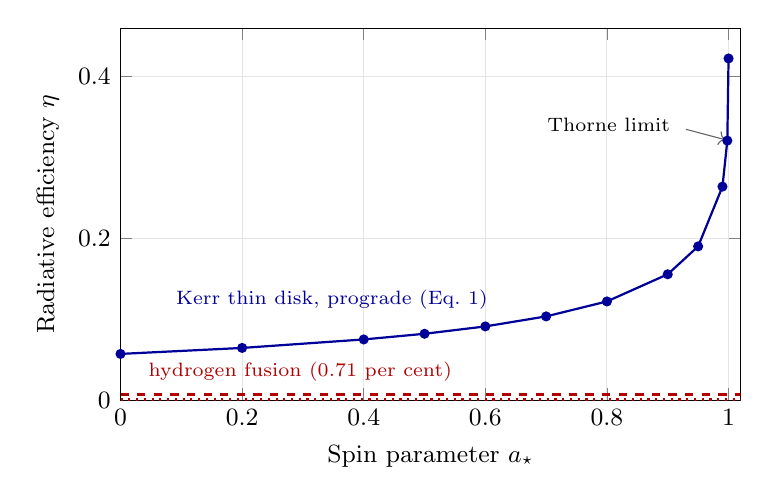
\begin{tikzpicture}
\begin{axis}[
  width=0.78\textwidth, height=0.52\textwidth,
  xlabel={Spin parameter $\astar$},
  ylabel={Radiative efficiency $\eta$},
  xmin=0, xmax=1.02, ymin=0, ymax=0.46,
  grid=both, grid style={black!10},
  tick label style={font=\small}, label style={font=\small}
]
\addplot[thick, blue!60!black, mark=*, mark size=1.4pt] coordinates {
 (0,0.0572) (0.2,0.0646) (0.4,0.0751) (0.5,0.0821) (0.6,0.0912)
 (0.7,0.1036) (0.8,0.1221) (0.9,0.1557) (0.95,0.1902)
 (0.99,0.2641) (0.998,0.3210) (1.0,0.4226)
};
\addplot[thick, dashed, red!70!black] coordinates {(0,0.0071)(1.02,0.0071)};
\addplot[thick, dotted, red!70!black] coordinates {(0,0.0007)(1.02,0.0007)};
\node[font=\scriptsize, text=blue!60!black, anchor=south east] at (axis cs:0.62,0.10) {Kerr thin disk, prograde (Eq.~1)};
\node[font=\scriptsize, text=red!70!black, anchor=south west] at (axis cs:0.03,0.011) {hydrogen fusion (0.71 per cent)};
\node[font=\scriptsize, text=red!70!black, anchor=north west] at (axis cs:0.40,0.0007) {Dyson lifetime yield (0.07 per cent)};
\node[font=\scriptsize, anchor=east] at (axis cs:0.92,0.34) {Thorne limit};
\draw[->, black!60] (axis cs:0.93,0.335) -- (axis cs:0.995,0.322);
\end{axis}
\end{tikzpicture}
\caption{Mass-to-energy conversion efficiency of thin-disk accretion as a function of black-hole spin \citep{BardeenPressTeukolsky1972,NovikovThorne1973}, compared with hydrogen fusion and with the lifetime yield of Dyson-type stellar harvesting. The \citet{Thorne1974} limit $\astar = 0.998$ marks the equilibrium spin reachable by disk accretion alone; the plotted $\eta \simeq 0.32$ there is the geodesic value, reduced to $\simeq 0.30$ once photon capture is included \citep{Thorne1974}. Curve drawn through exact values of Eq.~(\ref{eq:eta}) at the plotted points.}
\label{fig:efficiency}
\end{figure}

\paragraph{Power throughput.} The sustainable luminosity is bounded by the Eddington limit,
\begin{equation}
L_{\mathrm{Edd}} = \frac{4\pi G M m_p c}{\sigma_T} \simeq 1.26\times10^{31}\,\Bigl(\frac{M}{\msun}\Bigr)\ \mathrm{W},
\label{eq:edd}
\end{equation}
giving $1.0\times10^{35}$, $2.5\times10^{35}$, and $6.3\times10^{35}$~W at $M = 8.2\times10^{3}$, $2\times10^{4}$, and $5\times10^{4}\,\msun$ respectively \citep{FrankKingRaine2002,ShapiroTeukolsky1983}, some $3\times10^{8}$--$2\times10^{9}$ times the bolometric output of the Sun across that mass range ($6.6\times10^{8}$ at $2\times10^{4}\,\msun$), and hence of any solar Dyson swarm (Fig.~\ref{fig:power}). The corresponding Eddington accretion rate, $\dot M_{\mathrm{Edd}} = L_{\mathrm{Edd}}/\eta c^{2}$, is remarkably modest: at $\eta = 0.1$ and $M = 2\times10^{4}\,\msun$, one solar mass sustains the limit for $\sim$2,300 years. At $\omega$~Cen's adopted central density ($\sim$$3\times10^{3}\,\msun\,\mathrm{pc}^{-3}$; Table~\ref{tab:ocparams}) the central parsec holds $\sim$$1.3\times10^{4}\,\msun$, roughly $3\times10^{4}$ stars, or $\sim$$3\times10^{7}$~yr of Eddington fuel on its own; the working reservoir is the central $\sim$10~pc, whose $\sim$$10^{6}$ stars fuel Eddington-limited operation for $10^{8\text{--}9}$ years using bodies (brown dwarfs, low-mass M dwarfs, white dwarfs) that no fusion-based economy values, at the delivery cost priced in Section~\ref{sec:architecture}.

\begin{figure}[tbp]
\centering
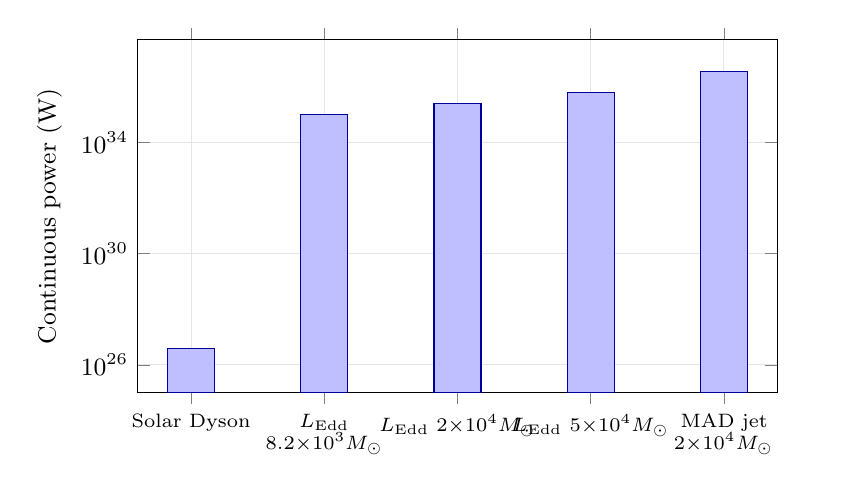
\begin{tikzpicture}
\begin{axis}[
  width=0.8\textwidth, height=0.5\textwidth,
  ybar, bar width=17pt,
  ymode=log, log origin=infty,
  ymin=1e25, ymax=5e37,
  ylabel={Continuous power (W)},
  symbolic x coords={Solar Dyson, {$L_{\rm Edd}$ $8.2{\times}10^3 M_\odot$}, {$L_{\rm Edd}$ $2{\times}10^4 M_\odot$}, {$L_{\rm Edd}$ $5{\times}10^4 M_\odot$}, {MAD jet $2{\times}10^4 M_\odot$}},
  xtick=data,
  x tick label style={font=\scriptsize, text width=2.1cm, align=center},
  tick label style={font=\small}, label style={font=\small},
  grid=major, grid style={black!10}
]
\addplot[fill=blue!25, draw=blue!60!black] coordinates {
 (Solar Dyson, 3.8e26)
 ({$L_{\rm Edd}$ $8.2{\times}10^3 M_\odot$}, 1.0e35)
 ({$L_{\rm Edd}$ $2{\times}10^4 M_\odot$}, 2.5e35)
 ({$L_{\rm Edd}$ $5{\times}10^4 M_\odot$}, 6.3e35)
 ({MAD jet $2{\times}10^4 M_\odot$}, 3.5e36)
};
\end{axis}
\end{tikzpicture}
\caption{Continuous power available to a civilization from a complete solar Dyson swarm versus Eddington-limited accretion (Eq.~\ref{eq:edd}) onto IMBHs spanning the contested $\omega$~Cen mass range, and a magnetically arrested (MAD) Blandford--Znajek jet at $\astar \simeq 0.99$ with $\eta_{\rm jet} \simeq 1.4$ \citep{Tchekhovskoy2011}, fed at the $\eta = 0.1$ Eddington rate; the two efficiency conventions combine as $P_{\rm jet} = \eta_{\rm jet}\,\dot M c^{2} = \eta_{\rm jet}\,(L_{\rm Edd}/\eta)$. The IMBH advantage in instantaneous power is roughly nine orders of magnitude.}
\label{fig:power}
\end{figure}

\paragraph{Spin energy and the Blandford--Znajek channel.} A Kerr hole stores extractable rotational energy
\begin{equation}
E_{\mathrm{rot}} = \Bigl[1 - \sqrt{\tfrac{1}{2}\bigl(1 + \sqrt{1-\astar^{2}}\bigr)}\,\Bigr] M c^{2},
\end{equation}
reaching $0.29\,Mc^{2} \simeq 1.0\times10^{51}$~J for $M = 2\times10^{4}\,\msun$ at $\astar \to 1$: a reservoir equal to the entire lifetime fusion output of $\sim$$10^{7}$ Suns, storable indefinitely and tappable on demand. The bracketed quantity is the Christodoulou--Ruffini reducible energy, the difference between $M$ and the irreducible mass $M_{\mathrm{irr}}$ \citep{Christodoulou1970,ChristodoulouRuffini1971}; extraction is reversible only in the limit of vanishing horizon-area increase, and inefficient extraction raises $M_{\mathrm{irr}}$ permanently, destroying future capacity, a distinction that matters for the spin-fossil reasoning of Section~\ref{sec:falsification}. That this energy is extractable in principle was shown by the ergosphere mechanism of \citet{Penrose1969} and \citet{PenroseFloyd1971}; the astrophysically efficient extraction mechanism is electromagnetic: a horizon threaded by poloidal magnetic flux $\Phi$ supplied by an accretion disk acts as a unipolar inductor, driving Poynting-flux jets with power $P_{\mathrm{BZ}} \propto \Phi^{2}\Omega_{H}^{2}$, where $\Omega_{H}$ is the horizon angular frequency \citep{BlandfordZnajek1977}. In the membrane paradigm of \citet{ThornePriceMacdonald1986} the horizon carries a surface resistivity of 377~$\Omega$ and the whole configuration reads as a battery with internal resistance, the engineering-facing form of the mechanism and the one relevant to Section~\ref{sec:architecture}'s power-station framing. In the magnetically arrested disk (MAD) regime, general-relativistic magnetohydrodynamic simulations find jet efficiencies $\eta_{\mathrm{jet}} \equiv P_{\mathrm{jet}}/\dot M c^{2} \simeq 1.4$ at $\astar \simeq 0.99$ \citep{Tchekhovskoy2011,Tchekhovskoy2015}: the jet carries more energy than the accreted rest mass, the excess drawn from spin. The BZ scaling has recently been confirmed from first principles by ab-initio particle-in-cell simulations of Kerr magnetospheres \citep{Meringolo2025}, which additionally identify equatorial magnetic reconnection as a supplementary extraction channel \citep{ComissoAsenjo2021,CamilloniRezzolla2025}; one 2026 preprint reports transient MAD states with jet power exceeding accretion power by over two orders of magnitude \citep[not yet peer-reviewed]{Nathanail2026}. For the MTH it suffices that $\eta_{\mathrm{jet}} \gtrsim 1$ is robust across methods: an engineered MAD configuration around a spun-up IMBH is, per unit fuel, the most efficient large-scale power plant permitted by demonstrated physics.

\paragraph{Spin-up economics.} A hole of low natal spin is itself improvable. Prograde thin-disk accretion drives $\astar \to 0.998$ after the hole grows by a factor $\approx 2.2$ ($2.2024$) \citep{Bardeen1970,Thorne1974}; for an initial $2\times10^{4}\,\msun$ hole this costs $\sim$$2.4\times10^{4}\,\msun$ of accreted matter (of order $10^{4\text{--}5}$ cluster stars) and, at Eddington throughput, $\sim$$3.5\times10^{7}$ years. The investment multiplies all subsequent per-unit-fuel returns by up to $\sim$6 (Fig.~\ref{fig:efficiency}) and unlocks the BZ reservoir. The corollary for observers: spin is a key parameter of the system's history (Section~\ref{sec:falsification}), since the MTH requires engineered systems to approach near-extremal spin; the converse inference is weaker, because some natural formation channels, in particular coherent disk growth in a gas-rich nucleus, also reach high spin \citep[Section~\ref{sec:falsification};][]{Reynolds2021}.

\subsection{Entropy disposal: the horizon as the ultimate cold reservoir}
\label{sec:landauer}

Landauer's principle sets the minimum thermodynamic cost of irreversible computation: erasing one bit dissipates at least $\kb T\ln 2$ into a reservoir at temperature $T$ \citep{Landauer1961,Bennett1982,Parrondo2015}, a bound verified experimentally \citep{Berut2012}. Reversible logic evades the bound for intermediate steps \citep{Bennett1973,Toffoli1980,FredkinToffoli1982,Frank2002,Athas1994}, but error correction, measurement, and memory reuse impose a residual erasure budget on any real computer \citep{Wolpert2019}. For a conventional deep-space computer the reservoir floor is the CMB at $T_{\gamma} = 2.7$~K, so the marginal cost is $\kb T_{\gamma}\ln 2 = 2.6\times10^{-23}$~J per bit. This is the floor that aestivation proposes to lower by waiting $\sim$$10^{12}$ years \citep{Sandberg2016}.

An event horizon lowers it in the present epoch. By the generalized second law (GSL), the sum of black-hole entropy $S_{\mathrm{BH}} = \kb c^{3}A/4G\hbar$ and exterior entropy is non-decreasing, and entropy carried across the horizon is accounted by the area increase \citep{Bekenstein1973,Bekenstein1974,Bousso2002}. A computation platform orbiting the hole may therefore dump its waste entropy into the horizon rather than radiating it to the sky. The marginal energy cost of horizon disposal is set by the horizon temperature
\begin{equation}
T_{H} = \frac{\hbar c^{3}}{8\pi G M \kb} \simeq 6.2\times10^{-8}\,\Bigl(\frac{\msun}{M}\Bigr)\,\mathrm{K},
\label{eq:hawking}
\end{equation}
\citep{Hawking1974,Hawking1975}: $T_H \simeq 3\times10^{-12}$~K at $2\times10^{4}\,\msun$, twelve orders of magnitude below the CMB. A bit dumped at the horizon costs $\kb T_H \ln 2 \sim 3\times10^{-35}$~J against $2.6\times10^{-23}$~J for CMB radiation (Fig.~\ref{fig:landauer}). In practical terms the erasure cost ceases to be the binding constraint on computation; the budget shifts to transport of waste heat to the horizon (radiative or conductive tethering from the ISCO swarm inward), an engineering loss rather than a thermodynamic floor. The quantified gain from this substitution is the $\sim 10^{12}$ temperature ratio between the CMB and the horizon; the larger $\sim 10^{30}$ factor cited by \citet{Sandberg2016} assumes cooling to temperatures far below the horizon temperature used here and is not directly comparable. The substitution's decisive property is that it operates without waiting, and therefore without forfeiting the free energy that \citet{Bennett2019} showed dormant civilizations irretrievably lose. The related configuration of \citet{Opatrny2017}, a shell absorbing CMB radiation as its hot reservoir and rejecting entropy to a central black hole, demonstrates the same thermodynamic asymmetry in a fully worked classical setting.

The claim should also be stated in its energy-conservation form, because that is where the mainstream objection lands. \citet{Curtis2026DysonMinds} state the standard position: Dyson-scale computation must reradiate nearly all of the energy it absorbs, so mid-infrared thermal emission is the robust technosignature of black-hole-hosted intelligence. For a horizon-sink architecture the premise fails, and it fails on energy grounds rather than entropy grounds: the waste carriers themselves cross the horizon, and their energy goes with the entropy. Writing $f_{\mathrm{sink}}$ for the fraction of waste \emph{energy} delivered into the capture cone (a vocabulary adopted throughout this series), only the missed fraction $(1-f_{\mathrm{sink}})$ must be reradiated, at swarm temperature; the absorbed remainder raises $M$ and thereby lowers $T_H$ further, so the channel is weakly self-improving. The disagreement with \citet{Curtis2026DysonMinds} is thus quantitative and falsifiable: the predicted mid-infrared residue scales with $(1-f_{\mathrm{sink}})$ rather than with the full computational throughput.

The $\kb T_H \ln 2$ figure is the marginal cost of \emph{disposal at the horizon}; it is not the delivered cost from an orbiting platform, and the gap between the two can be estimated rather than merely flagged. Consider radiative delivery, the least demanding channel. Efficient absorption requires a carrier wavelength $\lambda \lesssim r_g$, the geometric-optics condition for capture rather than diffraction around the hole (aiming is a separate and easier requirement, treated below). At $M = 2\times10^{4}\,\msun$, $r_g \simeq 3\times10^{7}$~m, so the vacuum-gravitational floor on the carrier energy is $E_\gamma \gtrsim hc/r_g \simeq 7\times10^{-33}$~J, corresponding to a frequency of $\sim$10~Hz. That floor is unreachable through plasma: propagation requires $\nu > \nu_p = 8.98\,\mathrm{kHz}\,\sqrt{n_e/\mathrm{cm}^{-3}}$, and even the cluster's ambient $n_e = 0.23\,\mathrm{cm}^{-3}$ gives $\nu_p \simeq 4.3$~kHz, while any fed inner-flow environment ($n_e \sim 10^{4}$--$10^{8}\,\mathrm{cm}^{-3}$ inside $\sim$$10^{2}\,r_g$) gives $\nu_p \simeq 1$--$90$~MHz. The minimum propagating carrier energy is therefore set by the plasma cutoff, at $\sim$$10^{-27}$--$10^{-26}$~J, three to six decades above $hc/r_g$. Two consequences follow. First, single-bit-per-photon delivery no longer suffices: at the plasma-cutoff carrier energy the advantage over the CMB would erode toward $10^{4}$--$10^{7}$. What preserves the realized range is dense coding: a carrier may bear many bits, up to the Bekenstein channel capacity \citep{Bekenstein1981,Bousso2002}, and coding at a modest fraction of capacity restores the delivered cost per bit to a factor of $10^{6}$--$10^{9}$ below the CMB figure of $2.6\times10^{-23}$~J. Second, matter carriers evade the cutoff entirely: cold mass dropped down the capture cone crosses the horizon with its entropy and energy aboard and no dispersion relation to satisfy, and serves as the fallback channel wherever the local plasma forbids cheap photons. Charging realistic engineering losses against these channels (pointing and capture inefficiency, error-correction overhead, the fraction of carriers scattered rather than absorbed) leaves a defensible realized gain of $\sim$$10^{6}$--$10^{9}$ over the 2.7~K sky. Gravitational bookkeeping does not change this range: energy accounted at a platform of radius $r \gtrsim 10^{2}\,r_g$ is redshifted at infinity by the platform's lapse factor, a $\approx$1 per cent correction at these radii. The realized economy therefore sits well above the $\kb T_H \ln 2$ floor and well below the CMB figure, and we quote $10^{6}$--$10^{9}$ rather than the floor-to-floor ratio of $\sim$$10^{12}$ wherever the realized gain is meant. An improvement of six orders of magnitude over the 2.7~K sky already dominates the aestivation trade.

Delivery geometry can be derived rather than assumed. The photon-capture cross-section of a Schwarzschild hole is $\sigma = \pi b_{\mathrm{crit}}^{2} = 27\pi r_g^{2}$, with critical impact parameter $b_{\mathrm{crit}} = 3\sqrt{3}\,r_g$; from a platform at $r = 10^{2}\,r_g$ the capture target subtends a solid-angle fraction $\Omega_c/4\pi = 6.75\times10^{-4}$, so isotropic emission delivers less than a thousandth of its power to the horizon. Reaching $f_{\mathrm{sink}} \to 1$ therefore requires a beaming gain $\gtrsim 1.5\times10^{3}$, which is optically trivial: the capture cone has half-angle $\theta_c \simeq 0.052$~rad, so diffraction demands only an aperture $D \gtrsim 23\lambda$, and the \'etendue (concentration) limit $1/\sin^{2}\theta_c \approx 3.7\times10^{2}$ puts the optic area at a few hundred times the radiator area. (The $27\pi r_g^{2}$ figure is the Schwarzschild value; the near-extremal prograde equatorial cross-section is somewhat smaller and anisotropic, an $O(1)$ correction.) The binding term in the delivery budget is re-interception within the swarm rather than aiming or aperture: beamed flux must traverse the swarm itself, and the intercepted fraction scales with the swarm covering fraction \citep{Swanson2026Engineered}.

\begin{figure}[tbp]
\centering
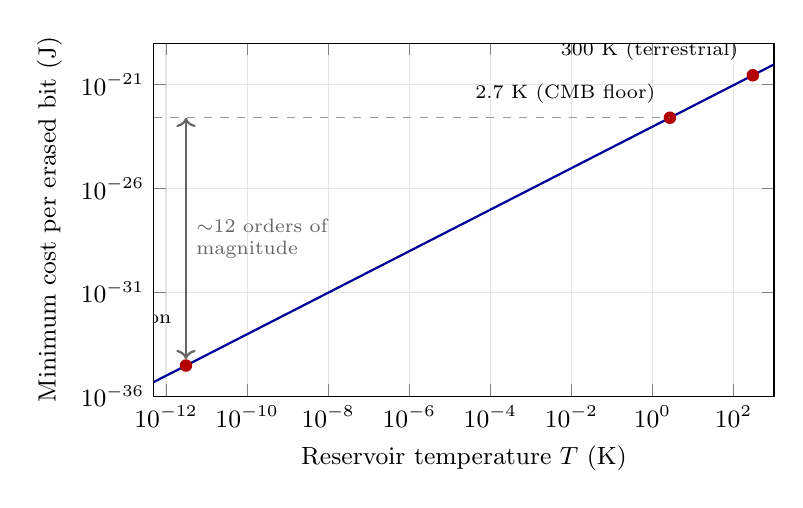
\begin{tikzpicture}
\begin{loglogaxis}[
  width=0.78\textwidth, height=0.5\textwidth,
  xlabel={Reservoir temperature $T$ (K)},
  ylabel={Minimum cost per erased bit (J)},
  xmin=5e-13, xmax=1e3, ymin=1e-36, ymax=1e-19,
  grid=both, grid style={black!10},
  tick label style={font=\small}, label style={font=\small}
]
\addplot[thick, blue!60!black, domain=5e-13:1e3, samples=2] {1.380649e-23*0.6931*x};
\node[circle, fill=red!70!black, inner sep=1.6pt, label={[font=\scriptsize]above left:{300 K (terrestrial)}}] at (axis cs:300,2.87e-21) {};
\node[circle, fill=red!70!black, inner sep=1.6pt, label={[font=\scriptsize]above left:{2.7 K (CMB floor)}}] at (axis cs:2.7,2.58e-23) {};
\node[circle, fill=red!70!black, inner sep=1.6pt, label={[font=\scriptsize, align=left]above left:{$T_H$, $2{\times}10^4\,M_\odot$ horizon\\ (Eq.~\ref{eq:hawking})}}] at (axis cs:3.1e-12,2.97e-35) {};
\draw[<->, black!60, thick] (axis cs:3.1e-12,2.58e-23) -- (axis cs:3.1e-12,6e-35)
  node[midway, right, font=\scriptsize, align=left] {$\sim$12 orders of\\ magnitude};
\draw[dashed, black!40] (axis cs:5e-13,2.58e-23) -- (axis cs:2.7,2.58e-23);
\end{loglogaxis}
\end{tikzpicture}
\caption{Landauer cost per erased bit, $\kb T \ln 2$, as a function of reservoir temperature. Dumping waste entropy across an IMBH horizon (marginal temperature $T_H$, Eq.~\ref{eq:hawking}) rather than radiating to the CMB lowers the erasure floor by $\sim$$10^{12}$, in the present epoch, consistent with the generalized second law \citep{Bekenstein1974}. The aestivation hypothesis \citep{Sandberg2016} sought a comparable-in-kind gain by waiting $\sim$$10^{12}$ years for cosmological cooling, to still lower assumed reservoir temperatures.}
\label{fig:landauer}
\end{figure}

\subsection{Information storage: the Bekenstein--Hawking archive}
\label{sec:storage}

The Bekenstein bound limits the information content of any bounded system \citep{Bekenstein1981,Casini2008}; black holes saturate it, with
\begin{equation}
\frac{S_{\mathrm{BH}}}{\kb \ln 2} \simeq 1.5\times10^{77}\,\Bigl(\frac{M}{\msun}\Bigr)^{2}\ \mathrm{bits},
\end{equation}
i.e.\ $\sim 6\times10^{85}$ bits at $2\times10^{4}\,\msun$ \citep{Bekenstein1973,Hawking1975,Lloyd2000}. That coefficient is the Schwarzschild value; since the architecture ends near-extremal, we quote one self-consistent pair: at $\astar = 0.998$ the Kerr horizon area per unit $M^{2}$ is $0.53\times$ Schwarzschild, so a $2\times10^{4}\,\msun$ hole at that spin stores $\approx 3\times10^{85}$ bits, and the factor-2.2 mass growth of the spin-up path (Section~\ref{sec:energy}) more than recovers the difference through the $M^{2}$ scaling. Information crossing the horizon is scrambled but, by unitarity, not destroyed; retrieval timescales via Hawking radiation are, however, of order the evaporation time, $\sim 10^{67}(M/\msun)^{3}$~yr \citep{Page1976}: the archive is functionally write-only. Black holes likewise saturate the Margolus--Levitin bound on processing rate, $2E/\pi\hbar$ operations per second \citep{MargolusLevitin1998,Lloyd2000}. We treat these saturation properties not as a usable disk drive but as the formal statement that no material technology can out-store or out-compute the object the civilization is already orbiting.

\subsection{Time dilation as an engineering parameter}
\label{sec:dilation}

A platform on a circular equatorial geodesic at radius $r$ around a Kerr hole runs slow relative to infinity by
\begin{equation}
\frac{d\tau}{dt} \;=\; \frac{\sqrt{1 - 3r_g/r + 2\astar (r_g/r)^{3/2}}}{1 + \astar (r_g/r)^{3/2}},
\label{eq:dilation}
\end{equation}
\citep{BardeenPressTeukolsky1972}: $d\tau/dt = \sqrt{1/2} \simeq 0.707$ at the Schwarzschild ISCO, falling to $\simeq 0.093$ (a factor $\sim$11) at the prograde ISCO for $\astar = 0.998$ (Fig.~\ref{fig:isco}). Larger factors require powered non-geodesic hovering at diverging thrust cost and are not usable by stable platforms. The $\sim$$11{:}1$ ceiling is set by the \citet{Thorne1974} spin-equilibrium limit $\astar = 0.998$ rather than by orbital stability: the ISCO proper-time ratio falls toward zero as $\astar \to 1$, and it is the accretion physics capping the spin that caps the dilation. A tiered swarm can therefore place archival and slow-integration processes deep (subjectively skipping across external time) and interactive processes high, with the choice of orbit acting as a clock-rate dial, a resource with no terrestrial analogue, though we note its strategic value (e.g.\ outwaiting external change) trades directly against responsiveness. The dial is two-way: viewed from outside, a deep tier both runs and receives $11\times$ slower in external time, so deep placement taxes bandwidth to, and coherence with, the shallow tier; and uplink photons arrive blueshifted by the same factor, each depositing $\sim$$11\times$ its emitted energy at the deep receiver.

\begin{figure}[tbp]
\centering
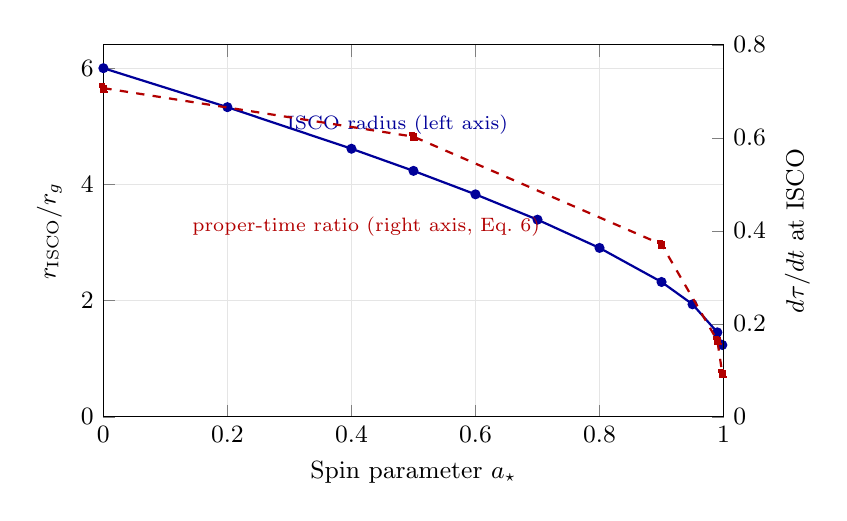
\begin{tikzpicture}
\begin{axis}[
  width=0.78\textwidth, height=0.52\textwidth,
  xlabel={Spin parameter $\astar$},
  ylabel={$r_{\mathrm{ISCO}}/r_g$},
  xmin=0, xmax=1.0, ymin=0, ymax=6.4,
  grid=both, grid style={black!10},
  tick label style={font=\small}, label style={font=\small},
  axis y line*=left
]
\addplot[thick, blue!60!black, mark=*, mark size=1.4pt] coordinates {
 (0,6.0) (0.2,5.329) (0.4,4.614) (0.5,4.233) (0.6,3.829)
 (0.7,3.393) (0.8,2.907) (0.9,2.321) (0.95,1.937) (0.99,1.454) (0.998,1.237)
};
\node[font=\scriptsize, text=blue!60!black, anchor=south west] at (axis cs:0.28,4.7) {ISCO radius (left axis)};
\end{axis}
\begin{axis}[
  width=0.78\textwidth, height=0.52\textwidth,
  xmin=0, xmax=1.0, ymin=0, ymax=0.8,
  axis y line*=right, axis x line=none,
  ylabel={$d\tau/dt$ at ISCO},
  tick label style={font=\small}, label style={font=\small}
]
\addplot[thick, dashed, red!70!black, mark=square*, mark size=1.3pt] coordinates {
 (0,0.7071) (0.5,0.6027) (0.9,0.371) (0.99,0.164) (0.998,0.0927)
};
\node[font=\scriptsize, text=red!70!black, anchor=north east] at (axis cs:0.72,0.45) {proper-time ratio (right axis, Eq.~6)};
\end{axis}
\end{tikzpicture}
\caption{Prograde ISCO radius (left axis) and proper-time ratio for a circular geodesic at the ISCO (right axis) as functions of spin \citep{BardeenPressTeukolsky1972}. Spin-up from $\astar=0$ to the Thorne limit moves the working orbit from $6\,r_g$ to $1.24\,r_g$ and deepens the available stable time dilation from $1.41{:}1$ to $\sim$$11{:}1$.}
\label{fig:isco}
\end{figure}

\subsection{Why inward beats outward for a computation-maximizer}
\label{sec:crossover}

The expansionist default implicitly maximizes resource acquisition; P1 civilizations maximize computation, and the two diverge. Expansion multiplies harvested mass polynomially in time ($\propto t^{3}$ for spherical growth at fixed speed) while imposing light-lag decoherence on any shared computation: a civilization spread over $10^{3}$ light-years cannot function as one computer on subjective timescales shorter than millennia. Concentration, by contrast, multiplies the yield per unit mass by the factors of Section~\ref{sec:energy} (up to $\sim$600 over Dyson harvesting without star lifting), lowers the realized erasure cost by $10^{6}$--$10^{9}$ (Section~\ref{sec:landauer}), and keeps the entire system within light-seconds of itself. We must be careful about what this establishes. An undiscounted maximizer of total integrated computation over unbounded time is served by expansion despite the per-unit-mass penalty, because controlled mass grows as $t^{3}$ and per-unit efficiency gains are bounded. The gradient points inward only under at least one of three auxiliary assumptions, which we adopt as part of P1: (i) temporal discounting, so that near-term computation outweighs the polynomial tail; (ii) a requirement that the computation be unified and latency-bound, so that light-lag decoherence caps the useful radius; or (iii) bounded planning horizons, within which the concentration factors dominate the $t^{3}$ growth. Under any of these, beamed-sail transport makes a cluster-hosted IMBH reachable at negligible marginal cost \citep{Lubin2016,Armstrong2013} and concentration wins. We stress the modesty of the claim actually needed: P1 requires only that some civilizations satisfy one of (i)--(iii) and follow the gradient. Expansionist and stay-at-home civilizations may coexist with migrators; the Fermi-relevant point is that the oldest and most capable optimizers, the very civilizations whose absence the paradox finds most puzzling \citep{Hanson2021}, are the ones the gradient captures.

\subsection{Why one hole rather than many}
\label{sec:whyone}

The comparison set for P2 must include a rival platform that the falsification program itself puts on the table: the dark remnant swarm of hypothesis $H_1$ (Section~\ref{sec:falsification}). Under $H_1$ the centre of $\omega$~Cen contains an extended $2$--$3\times10^{5}\,\msun$ component of stellar-mass black holes \citep{BanaresHernandez2025}, twelve times the mass of the fiducial $2\times10^{4}\,\msun$ IMBH. Because $L_{\mathrm{Edd}} \propto M$, the swarm's aggregate Eddington power is $\sim$$3.2\times10^{36}$~W against the IMBH's $2.5\times10^{35}$~W: on raw power the ``falsifying'' configuration is the better platform by a factor of $\sim$13, and a selection theory that ignored this would be assuming its conclusion. Table~\ref{tab:swarmcompare} prices the two configurations against the P2 axes.

\begin{table}[tbp]
\centering
\caption{One IMBH versus a same-order swarm of stellar-mass holes, priced on the P2 axes. The swarm column takes $2.5\times10^{4}$ holes of $10\,\msun$ (total $2.5\times10^{5}\,\msun$, the upper end of the \citealt{BanaresHernandez2025} extended component); the IMBH column takes the fiducial $2\times10^{4}\,\msun$. Storage and tidal entries are quoted as ratios (arb.\ units).}
\label{tab:swarmcompare}
\small
\begin{tabular}{p{4.2cm}p{2.9cm}p{3.4cm}p{2.2cm}}
\toprule
Figure of merit & One $2\times10^{4}\,\msun$ hole & $2.5\times10^{4}$ holes of $10\,\msun$ & Advantage \\
\midrule
Aggregate $L_{\mathrm{Edd}}$ & $2.5\times10^{35}$~W & $3.2\times10^{36}$~W & swarm, $13\times$ \\
Storage, $\sum S_i \propto \sum M_i^{2}$ & $4\times10^{8}$ & $2.5\times10^{6}$ & IMBH, $160\times$ \\
Sink depth, $T_H \propto M^{-1}$ & $3.1\times10^{-12}$~K & $6.2\times10^{-9}$~K & IMBH, $2000\times$ \\
ISCO tidal field, $\propto M^{-2}$ & 1 & $4\times10^{6}$ & IMBH, $4\times10^{6}$ \\
Latency across working system & ms (one orbit) & $\mu$s per hole; pc-scale between holes & IMBH \\
\bottomrule
\end{tabular}
\end{table}

The IMBH wins decisively on three of the four P2 axes and loses on the fourth. Storage scales as $\sum M_i^{2}$, so fragmenting the central mass into $2.5\times10^{4}$ holes of $10\,\msun$ costs a factor of 160 even against the twelvefold mass advantage. Sink depth scales as $T_H \propto M^{-1}$, a $2000\times$ edge for the IMBH, and the edge survives the delivery-level accounting of Section~\ref{sec:landauer}: the realized erasure economy tracks the delivered carrier cost rather than $T_H$ directly, and the vacuum carrier floor $hc/r_g$ is $1.3\times10^{-29}$~J for a $10\,\msun$ hole against $6.7\times10^{-33}$~J for the IMBH, the same $\sim$$2\times10^{3}$ ratio. The ISCO tidal field, $\propto M^{-2}$ at fixed $r/r_g$, is $4\times10^{6}$ times harsher at $10\,\msun$, excluding all but dust-scale hardware from the deep orbits where the dilation and efficiency gains live. And a computation distributed over the swarm pays parsec-scale light lag between nodes, against milliseconds across a single working orbit, failing the latency-bound condition of Section~\ref{sec:crossover} by construction. A computation-maximizer offered both configurations takes the single hole, and would pay a large premium to consolidate.

This derivation does real work in the falsification program. T3 (Table~\ref{tab:tests}) treats a LISA-resolved remnant swarm as a decisive falsifier, and this subsection is why: the swarm loses on storage, sink depth, and tides by two to six orders of magnitude, so a maximizer with gigayears of run of the cluster would not have left the central mass in that configuration. T3 is thereby a derived kill switch rather than a stipulated one.

% =====================================================================
\section{Omega Centauri as the optimal observational target}
\label{sec:omegacen}

\subsection{The cluster}

$\omega$~Centauri is the most massive Galactic globular cluster ($M_{\mathrm{cl}} \approx 4\times10^{6}\,\msun$, $\sim$$10^{7}$ stars; \citealt{Harris1996}), at a kinematic distance of $5.49 \pm 0.06$~kpc \citep{Haberle2025oMEGACatVI}, in $\sim$$2\sigma$ tension with the Gaia EDR3 parallax ($5.24\pm0.11$~kpc; \citealt{Soltis2021}), whose error budget is dominated by the parallax zero-point systematics discussed by those authors, and consistent with the combined catalogue value ($5.43\pm0.05$~kpc; \citealt{BaumgardtVasiliev2021}); nothing in this paper depends on the difference. It is anomalous among globular clusters in nearly every respect that matters here: it hosts multiple stellar populations spanning a broad metallicity range \citep{JohnsonPilachowski2010}, a mean stellar age of $12.08\pm0.01$~Gyr with an intrinsic spread of $0.75$~Gyr \citep{Clontz2024}, significant rotation, and an associated tidal stream \citep{Ibata2019}; the consensus interpretation is that it is the surviving nucleus of a dwarf galaxy accreted and stripped by the Milky Way \citep{HilkerRichtler2000,BekkiTsujimoto2019,Souza2026oMEGACatX}. Table~\ref{tab:ocparams} summarizes the parameters used in this paper.

For the MTH selection criteria of Section~\ref{sec:selection}, the stripped-nucleus origin matters twice over. First, nuclear star clusters are the environments most likely to form and retain IMBHs \citep{Greene2020}. Second, the age structure implies that any technological lineage arising anywhere in the progenitor dwarf (or in the early Milky Way) has had $\gtrsim$8~Gyr to locate, reach, and develop the system: at beamed-sail transit speeds of $0.1$--$0.2\,c$ \citep{Lubin2016}, crossing the Galaxy takes $\lesssim 10^{6}$ years, roughly eight thousand times shorter than the available window.

\begin{table}[tbp]
\centering
\caption{Adopted parameters for $\omega$~Centauri (NGC 5139).}
\label{tab:ocparams}
\small
\begin{tabular}{lll}
\toprule
Quantity & Value & Source \\
\midrule
Distance & $5.49 \pm 0.06$~kpc & \citet{Haberle2025oMEGACatVI} \\
Cluster mass & $\approx 4\times10^{6}\,\msun$ & \citet{Harris1996,BaumgardtVasiliev2021} \\
Stellar count & $\sim 10^{7}$ & \citet{Harris1996} \\
Mean stellar age & $12.08 \pm 0.01$~Gyr (spread 0.75~Gyr) & \citet{Clontz2024} \\
Origin & stripped dwarf-galaxy nucleus & \citet{HilkerRichtler2000,Ibata2019,Souza2026oMEGACatX} \\
Central density & $\sim 3\times10^{3}\,\msun\,\mathrm{pc}^{-3}$ & \citet{BaumgardtVasiliev2021}; cf.\ $\sim 10^{3}$ in \citet{PryorMeylan1993} \\
Declination & $-47.5^{\circ}$ & \citet{Harris1996} \\
\bottomrule
\end{tabular}
\end{table}

\subsection{The IMBH candidate and the mass tension}
\label{sec:tension}

Evidence for a central dark mass in $\omega$~Cen has accumulated for two decades, from integrated kinematics \citep{Noyola2008} through proper-motion modelling that initially yielded only upper limits at the $\sim$$10^{4}\,\msun$ level \citep{vanderMarelAnderson2010}, with stellar-mass black-hole subsystems long advanced as the alternative explanation \citep{Zocchi2019,BreenHeggie2013} and a systematic $N$-body survey concluding that no Galactic globular cluster, $\omega$~Cen included, required an IMBH at all \citep{Baumgardt2019}. The situation changed qualitatively when \citet{Haberle2024Nature}, using a proper-motion catalogue of 1.4 million stars built from over 500 HST epochs \citep{Haberle2024oMEGACatII}, identified seven stars within 3~arcsec of the cluster centre moving faster than the local escape velocity. Their velocities alone require a point mass $\geq 8{,}200\,\msun$; including acceleration limits on the same stars raises the lower bound to $21{,}100\,\msun$ at 99\,per cent confidence (main text of \citealt{Haberle2024Nature}).\footnote{The abstract of \citet{Haberle2024Nature} quotes only the velocity-only $8{,}200\,\msun$ limit; the $21{,}100\,\msun$ figure appears in the main text. A Nature \emph{Author Correction} (doi:10.1038/s41586-024-08017-4) fixes an equation typo and a right-ascension offset; the results are unaffected.} Independent $N$-body modelling finds that an IMBH grown in situ to $\sim$$5\times10^{4}\,\msun$ reproduces the present-day cluster structure and fast-star population \citep{GonzalezPrieto2025}.

Against this stands \citet{BanaresHernandez2025}: a joint analysis of stellar kinematics and timing accelerations of the cluster's millisecond pulsars that places a $3\sigma$ upper limit of $\sim$$6\times10^{3}\,\msun$ on any central point mass, favouring instead an extended central dark component of $\approx 2$--$3\times10^{5}\,\msun$, naturally interpreted as a centrally concentrated cluster of stellar remnants. The most recent joint MeerKAT--Parkes timing analysis, by contrast, finds its measurements insensitive to an IMBH in the $10^{3}$--$10^{4}\,\msun$ range and places a $90$\,per cent upper limit of $<10^{5}\,\msun$ on the central mass \citep{ColomiBernadich2026}, a bound compatible with both camps. The two leading results are formally inconsistent under each side's stated modelling assumptions, and the disagreement is unresolved at the time of writing (Table~\ref{tab:mass}). We take no side; for this paper, the tension is what makes the system valuable as a target. The MTH requires a genuine IMBH (P2), so the \citet{BanaresHernandez2025} scenario, if confirmed, falsifies the $\omega$~Cen application outright (one of several clean kill switches catalogued in Section~\ref{sec:falsification}). LISA can settle the question definitively, contingent on a suitable source being in-band during the mission: a single IMBH undergoing a compact-object inspiral yields resolvable extreme- or intermediate-mass-ratio-inspiral (EMRI/IMRI) signals with percent-level mass and spin measurement, whereas a remnant swarm yields a qualitatively different gravitational-wave signature \citep{AmaroSeoane2018,Babak2017,Colpi2024}.

The contingency deserves emphasis, because the per-cluster IMRI rate for a $\sim$$10^{4}\,\msun$ hole is uncertain by orders of magnitude, and the plausible outcome of a 4--10~yr mission is that no inspiral is caught in-band, in which case the gravitational-wave branch of Section~\ref{sec:falsification} returns ``inconclusive'' rather than a verdict (Fig.~\ref{fig:tree}, silence branch). Two mitigations exist. The dense fast-star environment resolved by \citet{Haberle2024Nature} raises the prior on close compact companions relative to a field IMBH, though it does not remove the rate uncertainty. More important, an inspiral is not the only LISA channel: \citet{Strokov2022} show that a Galactic-cluster IMBH can reveal itself through Doppler modulation of the gravitational-wave signal of an orbiting stellar-mass binary, a continuous signature that requires no merger event during the mission. This channel constrains the mass, though not the spin, so the decisive T5 measurement remains inspiral-contingent.

One element of the predicted dark population has now been observed directly. \citet{Whitaker2026BH2} report the astrometric detection of a $4.46^{+1.22}_{-1.01}\,\msun$ black hole with reported orbital elements $P = 94$~yr, $e=0.72$, $a = 31$~AU and a $\sim$$0.8\,\msun$ main-sequence companion,\footnote{We note without resolution that the reported elements are in mild internal tension: Kepler's third law with $a = 31$~AU and $M_{\mathrm{tot}} \simeq 5.3\,\msun$ gives $P \simeq 75$~yr; the reported period exceeds this Kepler-implied value by $\sim$25 per cent; reconciliation presumably lies within the quoted uncertainties on $a$ and the masses.} from HST astrometry spanning 2002--2023 combined with JWST imaging: the first confirmed stellar-mass black hole in $\omega$~Cen, and the first astrometric detection of one in any globular cluster. The detection confirms that the cluster forms and retains stellar-mass black holes, the population of which both sides of the mass tension require ($\sim$$10^{4}$ such remnants in the extended-component scenario; a formation reservoir in the IMBH-growth scenario), and it anchors the low-mass end of the central mass budget with an object whose parameters are measured rather than modelled.

\begin{table}[tbp]
\centering
\caption{Current constraints on the central dark mass of $\omega$~Cen. The kinematic lower bounds and the pulsar-timing upper bound are mutually inconsistent under stated assumptions; resolution is expected from LISA EMRI observations and continued astrometry.}
\label{tab:mass}
\small
\begin{tabular}{p{4.1cm}p{3.4cm}p{6.2cm}}
\toprule
Constraint & Value & Method / source \\
\midrule
Lower bound (velocities only) & $\geq 8{,}200\,\msun$ & 7 fast stars, HST proper motions \citep{Haberle2024Nature} \\
Lower bound (with accelerations) & $\geq 21{,}100\,\msun$ (99\%) & same stars, acceleration limits \citep{Haberle2024Nature} \\
$N$-body growth models & $\sim 4.7$--$5.1\times10^{4}\,\msun$ & cluster-evolution simulations \citep{GonzalezPrieto2025} \\
Upper bound (point mass) & $< 6\times10^{3}\,\msun$ ($3\sigma$) & stellar kinematics + MSP timing \citep{BanaresHernandez2025} \\
Favoured alternative & extended $2$--$3\times10^{5}\,\msun$ & same analysis \citep{BanaresHernandez2025} \\
Timing (joint MeerKAT--Parkes) & insensitive at $10^{3}$--$10^{4}\,\msun$; $< 10^{5}\,\msun$ (90\%) & MSP timing \citep{ColomiBernadich2026} \\
Historical upper limits & $\lesssim 10^{4}\,\msun$ (model-dep.) & HST proper motions \citep{vanderMarelAnderson2010}; see also \citet{Zocchi2019} \\
\bottomrule
\end{tabular}
\end{table}

\subsection{Electromagnetic silence}
\label{sec:silence}

Whatever occupies the centre of $\omega$~Cen, it is extraordinarily dark. The deepest radio observation of any globular cluster ($\sim$170~h with ATCA at 7.25~GHz, reaching an rms of 1.1~$\mu$Jy\,beam$^{-1}$) detects nothing at any proposed cluster centre, bounding the accretion efficiency of a putative IMBH at $\epsilon \lesssim 4\times10^{-3}$ of the Bondi rate ($3\sigma$; model-dependent, with $\approx$1~dex of systematic from the fundamental-plane conversion) \citep{Mahida2026}, the deepest point yet in the radio-limit framework established for globular clusters by the MAVERIC survey \citep{Tremou2018}. JWST NIRCam and MIRI photometry of the central field likewise finds no source with the spectral energy distribution of an accreting IMBH, with limits most constraining at the low-mass end of the allowed range \citep{Chen2025JWST}. The X-ray channel, the standard probe of quiescent accretion, agrees: a $\sim$291~ks Chandra exposure detects no central point source, limiting the unabsorbed luminosity to $L_X(0.5$--$7.0\,\mathrm{keV}) \lesssim 1.6\times10^{30}$~erg\,s$^{-1}$, an Eddington ratio of $\lesssim 10^{-12}$ for a $10^{4}\,\msun$ hole \citep{Haggard2013}. To our knowledge, no dedicated technosignature search of $\omega$~Cen has been conducted at any wavelength, although the commensal opportunity is unusually rich: $\omega$~Cen is a flagship MeerKAT pulsar-timing target, so every timing session is a potential commensal SETI epoch on the cluster for Breakthrough Listen's MeerKAT backend; the first dedicated globular-cluster SETI survey \citep[five northern clusters with FAST; $\omega$~Cen is inaccessible from FAST's latitude]{Huang2026} demonstrates both the feasibility and the current emptiness of this niche, and a Gaia-based phase-space anomaly metric over 79 Galactic globular clusters, in which NGC~5139 ranks among the dynamically most complex systems proposed for technosignature-oriented follow-up \citep{Huang2026Crystallization}, provides independent validation for treating globular-cluster anomalies as search targets.

The logic matters here: the MTH predicts electromagnetic silence (P3--P4), but silence is equally consistent with, and more parsimoniously explained by, a quiescent, gas-starved compact object in a relaxed, gas-poor old cluster, which we adopt as the null hypothesis $H_0$ throughout. Silence cannot confirm the MTH; only the discriminating residues of P4 can separate the hypotheses (Section~\ref{sec:falsification}).

\subsection{Why not Sagittarius A*?}
\label{sec:whynotsgra}

A natural objection: if bigger is better, the Galactic Centre hosts a $4.3\times10^{6}\,\msun$ hole \citep{GRAVITY2022,EHT2022SgrAI} with abundant fuel. Three of the four selection criteria of Section~\ref{sec:selection} disfavour it; the first is thermodynamic, the second and third strategic (per the register of claim~1, Section~\ref{sec:claims}). First, the storage and erasure advantages saturate at IMBH scale: nothing a maximizer needs scales usefully beyond $\sim$$10^{4\text{--}5}\,\msun$, while hazards do. Second, the Galactic Centre is the most dynamically violent environment in the Galaxy (ongoing star formation, supernovae, magnetar flares, stochastic accretion flares, and a dense population of perturbers), the opposite of a stable substrate for Gyr-scale infrastructure; $\omega$~Cen's relaxed core offers the same physics in a far quieter dynamical environment. Third, the claim structure matters, in the era-relative form of criterion 3: the Galactic Centre's gas and stars are the future fuel of natural astrophysics and of any fusion-era competitor, whereas a globular cluster's low-mass reservoir is uncontested by fusion-era economics and contested only among computation-maximizing lineages, the population P1 already conditions on; the premium therefore goes to early arrival rather than to contest avoidance. The MTH thus predicts that the preferred class is IMBHs in dense old clusters rather than supermassive holes, a distinctive and testable preference, since it directs attention at objects mainstream SETI has never examined.

% =====================================================================
\section{A staged exploitation architecture}
\label{sec:architecture}

\specbox{This section is speculative civilizational engineering. It is included not as prediction but because the falsification program of Section~\ref{sec:falsification} requires a concrete model of what would be observable at each stage. Each stage uses only physics established in Section~\ref{sec:thermo} plus engineering extrapolations that are individually defended in the cited literature; the conjunction is unargued-for and carries the usual burden of compounded speculation.}

We model the migration as five phases (Fig.~\ref{fig:phases}), parameterized for a civilization departing a planetary system $\sim$5~kpc from $\omega$~Cen.

\textbf{Phase 1 --- Scouts.} Gram-scale beamed-sail probes at $0.1$--$0.2\,c$ \citep{Lubin2016}, with photon-braking and magnetic-sail deceleration into the cluster halo; transit $\sim$$10^{5}$~yr. Objectives: resolve the IMBH-versus-swarm question in situ, map the rocky-body inventory, and emplace a deceleration relay for following waves. \emph{External signature: none detectable at interstellar range.}

\textbf{Phase 2 --- Self-replicating industry.} Kilogram-scale seed factories bootstrap exponentially from asteroidal material, following the NASA self-replicating-systems concept \citep{Freitas1982}; decades to centuries to $10^{3+}$ factory units and a relay laser. \emph{Signature: waste heat of order early-industrial --- far below detectability.}

\textbf{Phase 3 --- Compute swarm.} The main payload (substrate-independent minds, by this stage the default cargo; cf.\ \citealt{Smart2012}) arrives and assembles a free-flying compute swarm. While the hole is being fed, the swarm's inner working boundary sits at $\gtrsim 10^{2}\,r_g$ ($\sim$$3\times10^{6}$~km at $2\times10^{4}\,\msun$): the companion infrastructure analysis \citep{Swanson2026Engineered} finds that accretion-flow erosion excludes hardware inside $\sim$$30\,r_g$ of a fueled hole, and differential Lense--Thirring precession already excludes rigid formations at $10^{2}\,r_g$, so the swarm must be free-flying there in any case. Controlled star-lifting of brown dwarfs establishes a thin sub-Eddington disk; BZ extraction begins at low spin. Tiered orbits allocate clock rate (Section~\ref{sec:dilation}), though for an operating (fueled) system the stable dilation on offer at the $10^{2}\,r_g$ working boundary is modest, $d\tau/dt \simeq 0.985$; the deep-orbit clock rates of Fig.~\ref{fig:isco} become available only to dormant or archival elements around an unfueled hole. \emph{Signature: faint, soft accretion luminosity --- the one phase in which the system would be conventionally observable; at $\omega$~Cen, current limits already exclude an active Phase 3 fed above $\sim 4\times10^{-3}$ of the Bondi rate \citep{Mahida2026} or radiating above $\sim 10^{-12}$ of Eddington \citep{Haggard2013,Chen2025JWST}.}

\textbf{Phase 4 --- Spin-up.} Sustained prograde feeding ($\sim$$10^{4\text{--}5}$ stars over $\sim$$3.5\times10^{7}$~yr, $0.79$ Salpeter e-foldings to reach Thorne's radiation-limited $\astar = 0.998$ ($M_{f}/M_{i} \approx 2.2$) \citep{Bardeen1970,Thorne1974,Swanson2026Engineered}; Section~\ref{sec:energy}) drives $\astar \to 0.9$--$0.998$; the ISCO migrates inward by a factor $\sim$5 and jet efficiency crosses unity in MAD episodes; the fueled swarm holds its $\sim$$10^{2}\,r_g$ working boundary throughout \citep{Swanson2026Engineered}. \emph{Signature: episodic jet activity if imperfectly managed; high spin as a permanent record. Secular cluster-core depletion is a weaker observable than earlier drafts implied: the delivered $(3\text{--}4)\times10^{4}\,\msun$ is $\sim$24 per cent of the mass inside 2~pc but only $\sim$1 per cent of the mass inside the 10-pc reservoir the fuel census requires, the removed stellar mass reappears as central point mass so the total enclosed profile is preserved, and any deficit refills on the $\sim$4-Gyr core relaxation time \citep{Harris1996,Swanson2026Engineered}.} We flag the strongest hidden premise of the whole architecture here: Phases 3--5 presuppose institutional or goal stability over $10^{8}$~yr, longer than mammalian evolutionary history, and stellar feeding requires active orbit-shaping of individual stars with non-trivial delta-$v$ budgets. We know of no principled argument that either is achievable; the architecture is offered conditional on both.

The delta-$v$ can at least be priced to order of magnitude, and the pricing rules out two of the three options a reader might imagine. Delivering a star inward from a near-circular cluster orbit requires removing nearly all of its orbital angular momentum; the per-star impulse is of order the local orbital speed, tens of km\,s$^{-1}$ across the central 1--10~pc and growing with the radius of the $\sim$10-pc reservoir that the fuel census of Section~\ref{sec:selection} requires. The energy is not the obstacle (binding energy is released on the way down); the angular momentum is.

\textbf{Natural refilling does not supply the rate.} Phase 4 needs $10^{4\text{--}5}$ stars over $\sim$$3.5\times10^{7}$~yr, i.e.\ $\sim$$3\times10^{-4}$--$3\times10^{-3}$ stars yr$^{-1}$. Natural loss-cone refilling, which resonant relaxation drives near the influence radius \citep{RauchTremaine1996}, delivers stars to the hole at the tidal-disruption rate, $\sim$$10^{-8}$--$10^{-7}$~yr$^{-1}$ for IMBHs in evolved clusters and $\sim$$5\times10^{-8}$~yr$^{-1}$ in the $\omega$~Cen models of \citet{GonzalezPrieto2025} specifically \citep{Swanson2026Engineered}. The shortfall is four to five orders of magnitude. The natural channel is not a slower alternative to engineered delivery; it is not a fuel supply for this architecture at all, and essentially the whole Phase-4 budget must be actuated.

\textbf{Beamed-momentum tugs are excluded by the waste-heat ceiling.} Imparting $\Delta v \sim 10^{2}$~km\,s$^{-1}$ to the $\sim$$3\times10^{4}\,\msun$ that Phase 4 consumes costs $\sim$$3\times10^{44}$~J of kinetic work, $\sim$$7\times10^{2}\,L_\odot$ averaged over $3.5\times10^{7}$~yr, which fits inside the concealment budget with room to spare. Paying that momentum in photons does not: a photon tug needs $E = \Delta p\,c \simeq 1.8\times10^{48}$~J, or $\sim$$4.2\times10^{6}\,L_\odot$ sustained over the $3.5\times10^{7}$~yr episode, $5.6\times$ the ambient fuel ceiling and two and a half to three and a half orders of magnitude above the mid-infrared limits that already bound an operating system at $\omega$~Cen \citep{Swanson2026Engineered}. The photons are absorbed by the star being moved and reradiated at stellar temperature across the cluster, so there is nowhere to put them. Gravitational-assist sequencing among cluster stars, which uses other stars as momentum reservoirs and pays only actuator overhead, is the one scheme that survives its own thermal signature.

\textbf{Delivery geometry, not merely delivery rate, is what the spin fossil records.} Loss-cone stars arrive isotropically, and isotropic feeding random-walks a hole's spin rather than raising it (Section~\ref{sec:falsification}; \citealt{Swanson2026Engineered}). Coherent prograde delivery is therefore not an efficiency improvement on the natural channel but the only channel that produces the observable this paper treats as its decisive test. A full account (which stars, in what order, at what actuator cost, in what orbital orientation) has not been produced and remains the largest quantitative gap in this section.

\textbf{Phase 5 --- Endpoint.} Near-extremal spin; waste entropy disposed across the horizon (Section~\ref{sec:landauer}); residual stellar population dispersed or consumed. During fueled operation the swarm computes at the $\gtrsim 10^{2}\,r_g$ working boundary ($d\tau/dt \simeq 0.985$); if the system instead enters a dormant, unfueled archival mode, elements can descend to the near-ISCO orbits of Fig.~\ref{fig:isco} and bank the full $\sim$$11{:}1$ stable dilation. The system is nearly, but not perfectly, thermodynamically silent: transport losses in delivering waste entropy to the horizon impose a waste-heat floor $L_{\mathrm{waste}} \gtrsim 10^{-4}\,P_{\mathrm{comp}}$ \citep{Swanson2026Engineered}, so current JWST mid-infrared limits already bound the computational throughput of any operating Phase-5 system at $\omega$~Cen to $P_{\mathrm{comp}} \lesssim 10^{3\text{--}4}\,L_\odot$; there is no radio leakage, and the horizon temperature is in the picokelvin range (Eq.~\ref{eq:hawking}). The sole conjectured emission channel is burst-mode: if intractable computations are delegated to manufactured micro black holes per \citet{Dvali2023}, their evaporation yields high-energy neutrino and gamma-ray transients. We note for completeness that the formation of micro black holes from focused radiation may be blocked by Schwinger-limit pair production \citep{AlvarezDominguez2024,BreitWheeler1934,Schwinger1951}; this conclusion is contested \citep{Loeb2024Comment}, and the MTH does not depend on the channel --- it affects only the strength of prediction T6 below.

\begin{figure}[tbp]
\centering
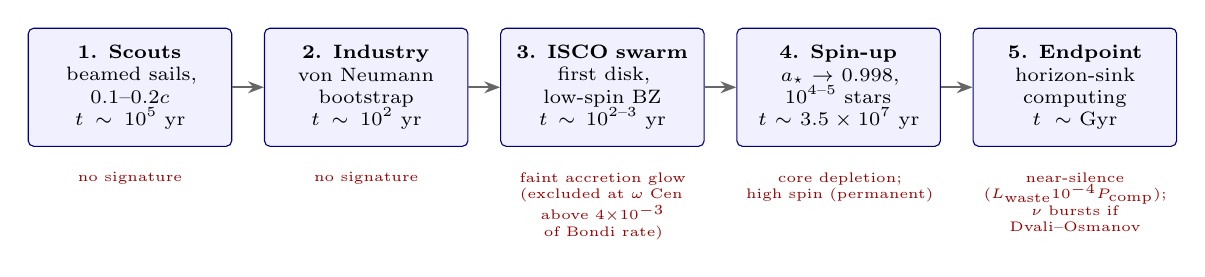
\begin{tikzpicture}[
  phase/.style={rectangle, rounded corners=2pt, draw=blue!50!black, fill=blue!6, text width=2.35cm, minimum height=1.5cm, align=center, font=\scriptsize},
  sig/.style={rectangle, text width=2.35cm, align=center, font=\tiny, text=red!60!black},
  arr/.style={-{Stealth[length=2mm]}, thick, black!60}
]
\node[phase] (p1) at (0,0) {\textbf{1. Scouts}\\ beamed sails, $0.1$--$0.2c$\\ $t \sim 10^{5}$ yr};
\node[phase] (p2) at (3.0,0) {\textbf{2. Industry}\\ von Neumann bootstrap\\ $t \sim 10^{2}$ yr};
\node[phase] (p3) at (6.0,0) {\textbf{3. ISCO swarm}\\ first disk, low-spin BZ\\ $t \sim 10^{2\text{--}3}$ yr};
\node[phase] (p4) at (9.0,0) {\textbf{4. Spin-up}\\ $a_\star\!\to\!0.998$, $10^{4\text{--}5}$ stars\\ $t \sim 3.5\times10^{7}$ yr};
\node[phase] (p5) at (12.0,0) {\textbf{5. Endpoint}\\ horizon-sink computing\\ $t \sim$ Gyr};
\draw[arr] (p1) -- (p2);
\draw[arr] (p2) -- (p3);
\draw[arr] (p3) -- (p4);
\draw[arr] (p4) -- (p5);
\node[sig, below=2mm of p1] {no signature};
\node[sig, below=2mm of p2] {no signature};
\node[sig, below=2mm of p3] {faint accretion glow\\ (excluded at $\omega$ Cen above $4{\times}10^{-3}$ of Bondi rate)};
\node[sig, below=2mm of p4] {core depletion;\\ high spin (permanent)};
\node[sig, below=2mm of p5] {near-silence ($L_{\rm waste} \gtrsim 10^{-4} P_{\rm comp}$);\\ $\nu$ bursts if Dvali--Osmanov};
\end{tikzpicture}
\caption{The five-phase exploitation architecture (speculative; see epistemic-status box) and the external signature of each phase. Only Phase 3 is conventionally luminous; the permanent observables are dynamical (spin, core depletion), which is why gravitational-wave spin measurement is the decisive test.}
\label{fig:phases}
\end{figure}

% =====================================================================
\section{Falsification framework and observational program}
\label{sec:falsification}

We define the competing hypotheses explicitly, then the tests.

\begin{description}
\item[$H_0$ (gas starvation; null).] The central object, whether IMBH or remnant swarm, is electromagnetically silent for the ordinary reason: a relaxed, gas-poor, 12-Gyr-old cluster supplies nothing to accrete. Favoured by parsimony and adopted as default.
\item[$H_1$ (dark remnant swarm).] No IMBH exists; the central mass is an extended cluster of stellar remnants \citep{BanaresHernandez2025,Zocchi2019,BreenHeggie2013}. Falsifies the $\omega$~Cen application of the MTH.
\item[$H_2$ (MTH).] An IMBH exists and is, or has been, the substrate of a migrated civilization (Section~\ref{sec:architecture}).
\end{description}

$H_0$ and $H_2$ predict identical electromagnetic appearances today (by design, since P3--P4 entail silence), so electromagnetic non-detections cannot distinguish them. They diverge on dynamical and high-energy observables. Table~\ref{tab:tests} states six tests with thresholds, instruments, and timelines; Fig.~\ref{fig:tree} arranges the decisive subset as a decision tree.

\begin{table}[tbp]
\centering
\caption{Falsification matrix for the MTH at $\omega$~Cen. ``Kills'' indicates what a positive result rules out; tests marked $\dagger$ are decisive against the hypothesis as a whole rather than against one phase. LISA timeline assumes launch in the mid-2030s \citep{Colpi2024}; T3--T5 are additionally contingent on a compact-object inspiral being in-band during the mission (Section~\ref{sec:tension}), with the Doppler-modulation channel of \citet{Strokov2022} providing a mass-only fallback.}
\label{tab:tests}
\scriptsize
\begin{tabular}{p{0.6cm}p{3.2cm}p{3.3cm}p{2.6cm}p{1.7cm}p{2.6cm}}
\toprule
\# & Observation & Threshold & Instrument & Timeline & Kills \\
\midrule
T1 & Accretion luminosity from core (limit-tightening) & Current best $L_{\rm acc} \approx 2.5\times10^{26}$~W ($\approx 10^{-9}L_{\rm Edd}$) \citep{Chen2025JWST}; near-term target one further decade, $\lesssim 10^{26}$~W. Supplementary trigger: sustained ($>1$~yr) brightening to $L_{\rm acc} > 10^{29}$~W & JWST MIRI; ATCA/ MeerKAT; Chandra & now--2030 & Each deepening null lowers the ceiling on managed accretion throughput; a brightening detection kills Phase 5 (managed environment). Bounds the accretion SED itself, where T2 bounds reradiated waste heat \citep{Haggard2013,Mahida2026} \\
T2 & Mid-IR waste-heat excess & $>3\sigma$ over stellar-population model, 10--25.5~$\mu$m (MIRI imaging limit); tested against the horizon-sink floor $L_{\rm waste} \gtrsim 10^{-4} P_{\rm comp}$ \citep{Swanson2026Engineered} & JWST MIRI & now--2030 & Any Dyson-type capture; deepening null tightens the ceiling on Phase 4--5 throughput (currently $P_{\rm comp} \lesssim 10^{3\text{--}4}\,L_\odot$) \\
T3$^\dagger$ & GW signature inconsistent with single point mass & stochastic background or multiple low-mass inspirals from core & LISA & late 2030s--2040s & $H_2$ entirely (confirms $H_1$); removes P2 substrate \\
T4 & EMRI point mass too small & clean chirp, $M < 5\times10^{3}\,\msun$ at $>3\sigma$ & LISA & late 2030s--2040s & The selection ranking of Section~\ref{sec:selection}: $\omega$~Cen would no longer be a P2-optimal destination, though a $5\times10^{3}\,\msun$ hole still delivers $\sim 6\times10^{34}$~W (Eq.~\ref{eq:edd}), so $H_2$ is weakened rather than excluded \\
T5$^\dagger$ & EMRI spin measurement low & $\astar < 0.1$ at $>3\sigma$ & LISA & late 2030s--2040s & The exploitation model: no BZ reservoir, no spin-up history; MTH survives only in unmodified ``pre-arrival'' form \\
T6 & High-energy neutrino bursts from core & $\geq 3$ tracks within $1^{\circ}$ in $10^{2\text{--}3}$~s, $E \gtrsim 10$~TeV, $>5\sigma$ post-trials, no astrophysical counterpart & KM3NeT/ARCA ($\omega$~Cen is up-going from the Mediterranean; dec.\ $-47^{\circ}$) & 2026--2035 & A null at full sensitivity closes the \citet{Dvali2023} channel; a detection is consistent with (not proof of) $H_2$ \\
\bottomrule
\end{tabular}
\end{table}

Three features of this matrix deserve emphasis. First, it contains genuine kill switches: T3 falsifies the $\omega$~Cen application outright, and T5 falsifies the only exploitation model we have offered; T4 is a demotion rather than a kill, removing $\omega$~Cen from the top of the P2 selection ranking while leaving a still-substantial power budget in place. The MTH cannot survive a confirmed remnant swarm or a non-spinning IMBH, except as vacuous speculation about other systems. Second, the LISA spin measurement is among the most informative numbers obtainable this generation (if an in-band inspiral delivers it; Section~\ref{sec:tension}), though both the natural-spin null and the expected yield must be stated carefully. Natural formation channels span the spin range \citep{Reynolds2021}: runaway stellar collisions build IMBHs near $10^{4}\,\msun$ without requiring rapid rotation of the remnant \citep{Fujii2024}, and incoherent minor-merger growth random-walks the spin toward a broad distribution centred near $\astar \approx 0.2$--$0.5$ \citep{Reynolds2021}, so the T5 trigger $\astar < 0.1$ occupies a small tail of the natural prior and the most probable natural outcome lands in the uninformative middle branch of Fig.~\ref{fig:tree}. A measured $\astar < 0.1$ still fires T5 cleanly; the hedge concerns how likely nature is to deliver a verdict, not what the verdict would mean. The paper's own account of $\omega$~Cen's origin (Section~\ref{sec:omegacen}) is, however, a gas-rich dwarf-galaxy nucleus, and an IMBH grown there by coherent disk accretion generically reaches high spin naturally; because Blandford--Znajek spindown at ambient fueling operates on $\sim$$4\times10^{11}$~yr timescales \citep{Swanson2026Engineered}, such natal spin survives to the present. A measured $\astar \gtrsim 0.9$ is therefore supporting evidence rather than a diagnostic residue on its own: the discriminating observation is the conjunction of high spin, electromagnetic silence far below the ambient Bondi supply, and the regulation signature of T1 (P4a--b together). EMRI parameter estimation at LISA delivers spin to better than percent precision for favourable systems \citep{Babak2017,AmaroSeoane2018}. Third, the program is cheap: T1--T2 are archival or piggyback analyses; T6 requires only a pointed monitoring program on an instrument already built for the southern sky \citep{AdrianMartinez2016,KM3NeT2025}, following the high-energy SETI logic of \citet{Lacki2025} and the pipeline practices of standard point-source searches \citep{IceCubePS2020}; the partially built ARCA array has already demonstrated discovery-class capability with the $\sim$220-PeV event KM3-230213A, the most energetic neutrino yet observed \citep{KM3NeT2025}; and T3--T5 are free by-products of LISA's planned EMRI science \citep{Colpi2024}.

The T6 burst criterion must clear the atmospheric-neutrino background, and an order-of-magnitude estimate shows it does under the stated cuts. Full-detector ARCA is expected to collect of order $10^{3}$ up-going atmospheric muon-neutrino events per year above 10~TeV over the full up-going sky \citep[effective areas and atmospheric fluxes from the KM3NeT~2.0 letter of intent;][]{AdrianMartinez2016}. A $1^{\circ}$-radius cone subtends $\sim$$10^{-3}$~sr, a fraction $\sim$$1.5\times10^{-4}$ of the up-going hemisphere, giving a source-cone rate of $\sim$0.15~events~yr$^{-1}$, i.e.\ $\lambda \sim 5\times10^{-9}$~s$^{-1}$. The Poisson expectation in a $10^{3}$~s window is then $\mu \sim 5\times10^{-6}$, so the probability of an accidental $\geq$3-fold multiplet per window is $\mu^{3}/6 \sim 2\times10^{-17}$; a decade of livetime contains $\sim$$3\times10^{5}$ independent $10^{3}$~s windows, for an expected false multiplet count of $\sim$$10^{-11}$ per decade. The $1^{\circ}$ cone is itself deliberately conservative: ARCA's track angular resolution above 10~TeV is $\sim$$0.1$--$0.2^{\circ}$, so a resolution-matched cone carries a background lower by a further factor of 25--100. The criterion is background-free by many orders of magnitude even allowing generous uncertainties in the effective area and a trials factor for scanning window durations; the practical limit on T6 is exposure, not background. A dedicated $\omega$~Cen technosignature campaign would be the first of its kind for any globular cluster beyond the pilot survey of \citet{Huang2026}, which could not observe $\omega$~Cen.

\begin{figure}[tbp]
\centering
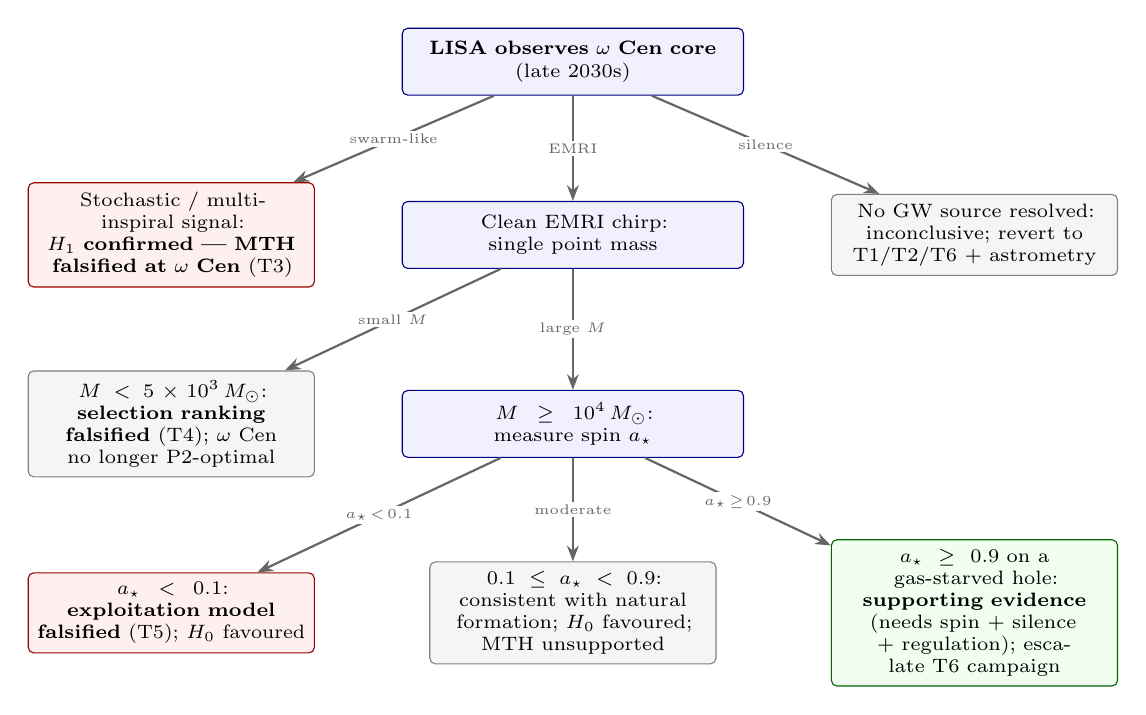
\begin{tikzpicture}[
  q/.style={rectangle, rounded corners=2pt, draw=blue!50!black, fill=blue!6, text width=4.1cm, align=center, font=\scriptsize, minimum height=0.85cm},
  o/.style={rectangle, rounded corners=2pt, draw=black!50, fill=black!4, text width=3.4cm, align=center, font=\scriptsize, minimum height=0.85cm},
  kill/.style={rectangle, rounded corners=2pt, draw=red!60!black, fill=red!6, text width=3.4cm, align=center, font=\scriptsize, minimum height=0.85cm},
  live/.style={rectangle, rounded corners=2pt, draw=green!40!black, fill=green!6, text width=3.4cm, align=center, font=\scriptsize, minimum height=0.85cm},
  arr/.style={-{Stealth[length=2mm]}, thick, black!60},
  lab/.style={font=\tiny, fill=white, inner sep=1pt}
]
\node[q] (lisa) at (0,0) {\textbf{LISA observes $\omega$ Cen core}\\ (late 2030s)};
\node[kill] (swarm) at (-5.1,-2.2) {Stochastic / multi-inspiral signal:\\ \textbf{$H_1$ confirmed --- MTH falsified at $\omega$ Cen} (T3)};
\node[q] (emri) at (0,-2.2) {Clean EMRI chirp:\\ single point mass};
\node[o] (nogw) at (5.1,-2.2) {No GW source resolved:\\ inconclusive; revert to T1/T2/T6 + astrometry};
\node[o] (small) at (-5.1,-4.6) {$M < 5\times10^{3}\,\msun$:\\ \textbf{selection ranking falsified} (T4); $\omega$~Cen no longer P2-optimal};
\node[q] (spin) at (0,-4.6) {$M \geq 10^{4}\,\msun$:\\ measure spin $\astar$};
\node[kill] (lowspin) at (-5.1,-7.0) {$\astar < 0.1$:\\ \textbf{exploitation model falsified} (T5); $H_0$ favoured};
\node[o] (midspin) at (0,-7.0) {$0.1 \leq \astar < 0.9$:\\ consistent with natural formation; $H_0$ favoured; MTH unsupported};
\node[live] (highspin) at (5.1,-7.0) {$\astar \geq 0.9$ on a gas-starved hole:\\ \textbf{supporting evidence} (needs spin + silence + regulation); escalate T6 campaign};
\draw[arr] (lisa) -- (swarm) node[lab, midway] {swarm-like};
\draw[arr] (lisa) -- (emri) node[lab, midway] {EMRI};
\draw[arr] (lisa) -- (nogw) node[lab, midway] {silence};
\draw[arr] (emri) -- (small) node[lab, midway] {small $M$};
\draw[arr] (emri) -- (spin) node[lab, midway] {large $M$};
\draw[arr] (spin) -- (lowspin) node[lab, midway] {$\astar\!<\!0.1$};
\draw[arr] (spin) -- (midspin) node[lab, midway] {moderate};
\draw[arr] (spin) -- (highspin) node[lab, midway] {$\astar\!\geq\!0.9$};
\end{tikzpicture}
\caption{Decision tree for the decisive (gravitational-wave) branch of the falsification program. Red boxes terminate the hypothesis or its exploitation model; the single green branch is the only outcome in which the MTH gains material support, and even there the inference is to ``anomaly requiring explanation,'' not detection.}
\label{fig:tree}
\end{figure}

\subsection{What would count as support}

Symmetry requires stating the confirmation side. The MTH gains support only from conjunctions that $H_0$ finds awkward: (i) a LISA-confirmed IMBH with $\astar \gtrsim 0.9$ in conjunction with Gyr-scale gas starvation and the regulation signature of T1, since high spin alone admits the natal-disk explanation above; (ii) repeated $>5\sigma$ neutrino bursts from the core with hard spectra and no electromagnetic counterpart, matching the \citet{Dvali2023} phenomenology; or (iii) a measured low-mass mass-function slope in the central 0.1~pc lying below the \citet{GonzalezPrieto2025} model envelope at $>3\sigma$ (oMEGACat photometry reaches the relevant depth), the concrete form of the P4c depletion residue. No single line, including all three jointly, would constitute proof of technology; they would constitute an anomaly stack justifying escalated scrutiny. Conversely, we commit in advance: if LISA delivers T3, T4, or T5, the $\omega$~Cen application of the MTH should be retired without special pleading.

% =====================================================================
\section{Discussion: objections and limits}
\label{sec:discussion}

\paragraph{Parsimony.} The MTH posits extraterrestrial intelligence; $H_0$ posits nothing. By any reasonable prior the null is favoured, and we have structured every comparison accordingly. The defensible claim is that the MTH is cheap to test relative to its information value, not that it is probable: it concentrates the diffuse question ``where is everybody?'' onto a handful of named objects and a decade-scale instrument schedule, and its decisive observables (IMBH reality, mass, spin) are independently first-rank astrophysics that will be measured anyway.

\paragraph{The anthropic objection.} If P1--P2 captured all civilizations, our own existence as a young, loud, planet-bound species is unremarkable; the MTH explains the silence of the old, not the existence of the young. It is therefore not undermined by our own counterexample, but neither can it explain why no expansionist civilizations are visible (cf.\ \citealt{Hanson2021}): if migration is optional, loud lineages should still exist somewhere. The defensible position is that the MTH thins the expected population of loud civilizations by removing its most capable members, sharpening rather than fully dissolving the paradox; full dissolution requires either high migration compliance or supplementary rarity from conventional Drake-equation factors.

\paragraph{Goal stability over $10^{8}$ years.} Phase 4 presupposes coherent purpose across timescales that dwarf all institutional experience. We flagged this as the architecture's largest unargued premise (Section~\ref{sec:architecture}). One partial mitigation: the architecture's payoff structure is front-loaded (Phase 3 already yields a substrate orders of magnitude beyond planetary computing), so a lineage that fragments mid-program still leaves durable traces, but fewer than we once supposed. The companion analysis \citep{Swanson2026Engineered} finds that an abandoned swarm is not preserved: collisional cascade grinds it to debris within $10^{2\text{--}3}$~yr, and the debris drains into the hole. The durable residues of incoherence are the spin acquired before fragmentation and, if Phase 4 ran long enough, the core depletion it caused; the hardware itself leaves no fossil. The observational program is robust to civilizational incoherence only through those two channels, which is a further reason the dynamical tests (T3--T5) carry the weight.

\paragraph{Tidal and radiative survivability at the ISCO.} At $2\times10^{4}\,\msun$ the tidal field at the Schwarzschild ISCO is $2GM/r_{\mathrm{ISCO}}^{3} \simeq 1$~s$^{-2}$: a 10-m node experiences a benign $\sim$$1\,g$ differential, while kilometre-scale rigid structures would face $\sim$$10^{2}\,g$ --- one reason the architecture assumes a swarm of small free-flying nodes rather than a monolithic platform. Radiation from even a managed accretion disk is the harsher constraint, and motivates the tiered-orbit design and sub-Eddington feeding discipline assumed in Section~\ref{sec:architecture}. We have not engineered these systems in detail and do not pretend to; the claim defended is the thermodynamic gradient (P2), not any specific machine.

\paragraph{Why has nothing arrived here?} A migration hypothesis must explain why migrators' probes are not conspicuous in every system, reviving \citet{Hart1975} and \citet{Tipler1980}. The MTH answer is economic: for a computation-maximizer, planetary systems are at most transit infrastructure rather than destinations; the Galaxy's uncollected starlight (an integrated stellar luminosity of $(1$--$2)\times10^{37}$~W) dwarfs any single system's output by ten orders of magnitude, and yet (Section~\ref{sec:crossover}) the marginal value of any outward claim is dominated by deepening the home gravity well. Quiet, minimal, purpose-built transit, rather than occupation, is the predicted footprint, consistent with the null results of artefact SETI to date \citep{Wright2022}. \citet{Ivliev2026} presses the opposite conclusion: once autonomous machine industry matures, outward expansion becomes too cheap and too useful for any civilization to refuse, and the attractor is quiet distributed expansion rather than concentration. We accept the premise that expansion is cheap, and we concede that for an undiscounted maximizer of total integrated computation Ivliev's inference goes through, since controlled mass grows as $t^{3}$. The disagreement localizes to the auxiliary assumptions of Section~\ref{sec:crossover}: under temporal discounting, latency-bound unified computation, or bounded planning horizons, expansion does not compete with concentration in yield per unit of controlled resource, and it is civilizations satisfying at least one of those conditions that the MTH captures. The two proposals are nonetheless observationally adjacent, since both predict a Galaxy free of conspicuous macro-engineering, and they diverge where the MTH is testable: Ivliev's filter predicts no privileged loci, while the MTH concentrates its residues on a short list of named systems.

\paragraph{The kugelblitz weak link.} The only positive high-energy signature we predict (T6) inherits the controversy over micro-black-hole formation from radiation \citep{AlvarezDominguez2024,Loeb2024Comment}. We therefore weight T6 as the cheapest test, not the strongest: its null closes a speculative channel; its detection would be extraordinary but stands or falls with \citet{Dvali2023} physics, not with the MTH core.

\paragraph{Scope of the $\omega$~Cen bet.} The MTH is a selection theory over a class; $\omega$~Cen is its highest-ranked accessible member, not its definition. Falsification at $\omega$~Cen (T3, or the ranking demotion of T4) retires the flagship application and substantially weakens the hypothesis (the Galaxy's best candidate failing is evidence about the class), but formally the theory survives in 47~Tuc, M54, and extragalactic nuclear clusters. We accept the methodological hazard this creates (unfalsifiability by retreat) and therefore bind ourselves to the class-level prediction: \emph{if no Galactic globular-cluster IMBH with $\astar \gtrsim 0.9$ exists, the MTH is wrong for the Milky Way}, a statement LISA-era gravitational-wave astronomy can settle.

% =====================================================================
\section{Conclusion}
\label{sec:conclusion}

We have argued, first as a matter of established physics, that rapidly spinning massive black holes in dense old stellar clusters constitute the global optimum among present-day environments for long-term computation (by factors of $\sim$$10^{2}$ in energy per unit fuel, $\sim$$10^{9}$ in continuous power, a realized $10^{6}$--$10^{9}$ in entropy-disposal cost once delivery overheads are charged against the $\sim$$10^{12}$ floor-to-floor ratio (Section~\ref{sec:landauer}), and unbounded factors in archival density), and second, as an explicitly speculative hypothesis, that this gradient acts on the oldest technological civilizations as an attractor whose operation would look, from outside, like the silence we observe. The Macro Transcension Hypothesis inherits the thermodynamic insight of transcension and aestivation while repairing their respective defects: it needs no exit from the universe and no dormancy, and it survives the \citet{Bennett2019} free-energy objection by importing the cold reservoir into the present rather than waiting for one.

Its principal virtue is that it pays its way observationally. The hypothesis selects a named target (Omega Centauri, whose contested $8\times10^{3}$--$5\times10^{4}\,\msun$ central object, perfect electromagnetic silence, and 12-Gyr head start make it scientifically urgent on entirely conventional grounds) and commits to kill criteria that existing and funded instruments will adjudicate: LISA's resolution of the IMBH-versus-swarm question and, above all, its spin measurement; deep accretion and waste-heat limits from JWST and southern radio arrays; and a first-of-its-kind neutrino monitoring campaign with KM3NeT. If the central object proves to be a remnant swarm, a light point mass, or a slowly spinning hole, the hypothesis fails at its flagship and we have said so in advance. If instead the 2030s deliver a massive, gas-starved, near-extremally spinning black hole in the quietest old cluster in the sky, the question this paper poses will have earned the right to be taken seriously.

% =====================================================================
\section*{Acknowledgements and disclosure}

The author thanks the maintainers of the NASA Astrophysics Data System and arXiv, on which the citation verification for this work relied. \textbf{AI assistance disclosure:} drafting, citation verification, derivation checking, and figure preparation for this manuscript were performed with substantial assistance from a large language model (Claude, Anthropic), under the author's direction; the author reviewed and takes full responsibility for all claims, derivations, and references. Interactive calculators implementing the quantitative material in Sections~\ref{sec:thermo}--\ref{sec:falsification} are available as supplementary material at \url{https://omegacentauri.me}.

\section*{Data availability}

No new observational data were generated. All cited measurements are available in the referenced publications.

% =====================================================================
\bibliographystyle{apalike}
\bibliography{references}

\end{document}
